\documentclass[12pt,a4paper]{report}

% ==================== PAQUETES ====================
\usepackage[spanish,activeacute]{babel} % Traducción automática al español
\addto\captionsspanish{
    \renewcommand{\tablename}{Tabla}
}
\usepackage[utf8]{inputenc} % Codificación UTF-8
\usepackage{amsmath,amssymb,amsfonts,amsthm} % Matemáticas AMS
\usepackage{mathtools,blkarray,esvect,cancel} % Extensiones matemáticas
\usepackage{bbold,bbm,latexsym} % Símbolos matemáticos
\usepackage{wasysym,eurosym,pifont,slashed,braket} % Símbolos especiales
\usepackage{setspace,multicol,soul,changepage} % Formato y maquetación
\usepackage{enumerate,enumitem,scrextend,blindtext} % Listas y utilidades
\usepackage{graphicx,float,wrapfig,caption} % Figuras e imágenes
\usepackage{multirow,longtable,color} % Tablas y colores
\usepackage{hyperref,pdfpages} % Hipervínculos y PDFs
\usepackage{subfiles,appendix,fancyhdr,geometry} % Estructura del documento
\usepackage{titlesec} % Formato de títulos
\usepackage{transparent} % Transparencia imagenes
\usepackage{tcolorbox} % color a cajas
\usepackage{tikz}
\usetikzlibrary{positioning,arrows.meta}
\usepackage{float}
\usepackage{listings}
\usepackage{xcolor}
\usepackage{lmodern}
\usepackage{subcaption}

% ==================== CONFIGURACIÓN ====================
\geometry{left=2.5cm,right=2.5cm,top=2.5cm,bottom=2.5cm}
\onehalfspacing
\pagestyle{fancy}
\fancyhf{}
\fancyfoot[C]{\thepage}
\setlength{\parskip}{0.4em}
\setlength{\parindent}{15pt}

% ==================== TÍTULOS ====================
\titleformat{\chapter}
{\bfseries\fontsize{16}{18}\selectfont}{\thechapter.}{1em}{}
\titleformat{\section}
{\bfseries\fontsize{14}{16}\selectfont}{\thesection}{1em}{}
\titleformat{\subsection}
{\bfseries\fontsize{12}{14}\selectfont}{\thesubsection}{1em}{}

% ==================== DOCUMENTO ====================
\begin{document}

% ==================== PORTADA ====================
\begin{titlepage}
\thispagestyle{empty}
\vspace*{-1.5cm}
\noindent
\includegraphics[width=0.18\textwidth]{./logos/logocolor.png}
\hfill
\raisebox{0.6cm}{
\includegraphics[width=0.18\textwidth]{./logos/membrete.jpeg}
}
\vspace{1cm}
\begin{center}
{\Large \textbf{MÁSTER EN ESTADÍSTICA APLICADA}}\\
\vspace{0.8cm}
{\Large {TRABAJO FIN DE MÁSTER}}\\
\vspace{0.8cm}
{\Huge \textbf{Análisis comparativo de la Regresión por Mínimos Cuadrados Parciales (PLS) en escenarios de Alta dimensionalidad y Multicolinealidad}}\\

\vspace{0.8cm}
{\large Presentado por:}\\
\vspace{0.3cm}
{\Large \textbf{Andrés Alejandro Ystúriz Caldeira}}\\
\vspace{0.5cm}
{\large Tutora:}\\
\vspace{0.3cm}
{\Large \textbf{Prof. Dra. Rocío Raya Miranda}}
\end{center}
\vfill

\begin{center}
{\transparent{0.25}
\includegraphics[width=0.5\textwidth]{./logos/logogris.png}
}
\end{center}
\vfill
\begin{center}
{\large Curso 2025 / 2026}
\end{center}

\end{titlepage}

% ==================== ORIGINALIDAD ====================
\thispagestyle{empty}

\begin{center}
    \includegraphics[width=4cm]{./logos/logocolor.png}

    \vspace{0.2cm}

\end{center}

\vspace{0.8cm}


%=========================
% CAJA TÍTULO
%=========================

\begin{center}
\begin{tikzpicture}
\node[
    draw=red!40,
    line width=0.5pt,
    minimum width=14cm,
    minimum height=1.2cm,
    align=center
]
{
\textbf{DECLARACIÓN DE AUTORÍA Y ORIGINALIDAD}\\
\textbf{DE TRABAJO FIN DE MÁSTER}
};
\end{tikzpicture}
\end{center}


\vspace{0.5cm}


\onehalfspacing

\noindent
\textbf{ANDRES ALEJANDRO YSTURIZ CALDEIRA} con NIE nº \textbf{Y6333991N}, 
estudiante del Máster Universitario en \textbf{Estadística Aplicada}, 
en relación con el Trabajo Fin de Máster \textit{Análisis comparativo de la Regresión por Mínimos Cuadrados Parciales (PLS) en escenarios de Alta dimensionalidad y Multicolinealidad}, presentado en la convocatoria de \textbf{2025 / 2026} declara que asume la originalidad de dicho 
trabajo, entendida en el sentido de que no ha utilizado fuentes sin 
citarlas debidamente.


\vfill


\noindent\makebox[\textwidth][c]{%
\includegraphics[
    width=\dimexpr\paperwidth-3cm\relax,
    keepaspectratio
]{./logos/Informacion_proteccion.png}
}

\newpage
% ==================== ÍNDICE ====================
\setcounter{page}{1}
\pagenumbering{roman}
\tableofcontents

\clearpage

\listoffigures

\clearpage

\listoftables

\newpage

% ==================== RESUMEN ====================
\cleardoublepage
\chapter*{Resumen}

Este Trabajo Fin de Máster analiza el comportamiento de la regresión por Mínimos Cuadrados Parciales (PLS) en escenarios caracterizados por multicolinealidad y alta dimensionalidad, comparando su rendimiento frente a diferentes métodos de regresión lineal. El estudio se motiva por la creciente presencia de conjuntos de datos complejos en áreas como la espectroscopía y la bioinformática, donde el elevado número de predictores y la fuerte correlación entre variables pueden limitar la aplicación de modelos clásicos.

El trabajo desarrolla una revisión teórica de la regresión PLS como una metodología basada en la construcción de componentes latentes que maximizan la covarianza entre las variables predictoras y la variable respuesta. Se estudian sus fundamentos matemáticos, los principales algoritmos de estimación, NIPALS y SIMPLS, así como su relación con otros enfoques destinados a tratar problemas de multicolinealidad y alta dimensionalidad, incluyendo Ridge, Lasso y la regresión por Componentes Principales (PCR).

Desde el punto de vista computacional, se implementa un entorno de análisis reproducible mediante un paquete modular desarrollado en Python, que integra las diferentes etapas del proceso experimental: preprocesamiento de datos, ajuste de modelos, selección de hiperparámetros, validación cruzada y evaluación predictiva. Esta arquitectura permite comparar los distintos métodos bajo un marco homogéneo y garantizar la trazabilidad de los resultados obtenidos.

La evaluación empírica se realiza utilizando tres conjuntos de datos reales con características diferenciadas: Tecator, Gasoline y Riboflavin. Estos permiten estudiar el comportamiento de los modelos en escenarios que van desde datos espectrales con fuerte estructura latente hasta problemas de alta dimensionalidad extrema donde el número de variables supera ampliamente al número de observaciones.

Los resultados obtenidos muestran que no existe un único método óptimo para todos los escenarios, sino que el rendimiento depende de la estructura interna del problema. PLS presenta un comportamiento especialmente competitivo cuando existe una fuerte correlación entre predictores y una estructura latente relacionada con la respuesta, destacando en problemas espectrales. Por otro lado, OLS puede mantener un buen rendimiento en situaciones donde la dimensionalidad es moderada, mientras que los métodos basados en regularización, especialmente Lasso, resultan más adecuados en contextos de alta dimensionalidad extrema con estructuras dispersas.

En conjunto, este trabajo confirma la importancia de seleccionar la técnica de regresión considerando las características de los datos y no únicamente el número de predictores disponibles. Asimismo, evidencia el valor de PLS como una herramienta robusta para la reducción supervisada de dimensionalidad y la construcción de modelos predictivos en presencia de multicolinealidad.

\vspace{0.5cm}

\textbf{Palabras clave:} regresión PLS, multicolinealidad, alta dimensionalidad, regularización, PCR, aprendizaje supervisado.

\cleardoublepage
\chapter*{Abstract}

This Master’s Thesis analyzes the behavior of Partial Least Squares Regression (PLS) in scenarios characterized by multicollinearity and high dimensionality, comparing its performance against different linear regression methods. The study is motivated by the increasing presence of complex datasets in fields such as spectroscopy and bioinformatics, where a large number of predictors and strong correlations between variables may limit the applicability of classical regression models.

The work provides a theoretical review of PLS regression as a methodology based on the construction of latent components that maximize the covariance between predictors and the response variable. Its mathematical foundations, the main estimation algorithms, NIPALS and SIMPLS, and its relationship with alternative approaches for handling multicollinearity and high-dimensional data, including Ridge, Lasso and Principal Component Regression (PCR), are discussed.

From a computational perspective, a reproducible analysis framework is implemented through a modular Python package that integrates the main stages of the experimental workflow: data preprocessing, model fitting, hyperparameter selection, cross-validation and predictive evaluation. This architecture enables a consistent comparison of the different methods while ensuring traceability and reproducibility of the results.

The empirical evaluation is carried out using three real datasets with different characteristics: Tecator, Gasoline and Riboflavin. These datasets allow the analysis of model performance across scenarios ranging from spectral data with strong latent structures to extreme high-dimensional problems where the number of variables greatly exceeds the number of observations.

The results show that there is no single optimal method for all situations, as performance strongly depends on the underlying data structure. PLS provides highly competitive results when predictors are strongly correlated and a relevant latent structure exists, particularly in spectral applications. In contrast, OLS may remain effective in moderate-dimensional settings, while regularization methods, especially Lasso, are more suitable for extreme high-dimensional problems with sparse structures.

Overall, this study highlights the importance of selecting regression techniques according to the characteristics of the data rather than only considering the number of available predictors. It also confirms the value of PLS as a robust tool for supervised dimensionality reduction and predictive modeling in the presence of multicollinearity.

\vspace{0.5cm}

\textbf{Key words:} PLS regression, multicollinearity, high dimensionality, regularization, PCR, supervised learning.



% ==================== CAPÍTULOS ====================
\fancyhead[L]{\nouppercase{\leftmark}}
\fancyfoot[C]{\thepage}
\chapter{Introducción}
\pagenumbering{arabic}
Cuando se hacen análisis de datos en contextos donde el número de variables explicativas es elevado, se plantean dificultades específicas asociadas a la presencia de relaciones de dependencia entre predictores. En áreas como la quimiometría, la bioinformática o la espectroscopía, esta situación suele generar problemas de multicolinealidad que afectan la estabilidad y la interpretabilidad de los modelos de regresión. Tal como indican Mateos‑Aparicio Morales y Caballero Domínguez, “el problema de la multicolinealidad [...] produce situaciones de inestabilidad de los coeficientes de regresión” \cite{mateos2007}, lo que evidencia una necesidad de utilizar métodos capaces de manejarse en escenarios con alta correlación entre variables.

La regresión por mínimos cuadrados ordinarios (\textit{Ordinary Least Squares} - OLS) constituye el punto de partida natural por su simplicidad y sus propiedades en los términos clásicos, sin embargo, presenta limitaciones claras cuando los predictores están altamente correlacionados o cuando la dimensionalidad del problema es elevada. La matriz \(X^\top X\) puede volverse casi singular o no ser invertible, generando estimaciones inestables y sensibles al ruido, con un impacto directo sobre la capacidad predictiva del modelo \cite{hastie2009, samosir2022}.

Para abordar estas limitaciones, se han desarrollado métodos basados en regularización y reducción de dimensionalidad. Entre ellos destacan Ridge y Lasso, que estabilizan las estimaciones mediante penalizaciones $L_2$ y $L_1$, respectivamente, y la regresión por componentes principales (\textit{Principal Component Regression} - PCR), que proyecta los predictores en un subespacio de menor dimensión \cite{hastie2009}. Estas técnicas permiten obtener estimaciones más estables y robustas frente a la correlación entre predictores.

Dentro de este conjunto de métodos, la regresión por mínimos cuadrados parciales (\textit{Partial Least Squares} - PLS) ocupa un lugar destacado por integrar reducción de dimensionalidad y orientación predictiva. A diferencia de PCR, PLS incorpora explícitamente la relación entre $X$ e $Y$, para así maximizar la covarianza entre ambas matrices \cite{geladi1986}. Este enfoque ha llevado a que PLS sea considerado “the workhorse of chemometrics” \cite{geladi1986}, especialmente cuando hay problemas donde resulta necesario extraer información predictiva a partir de estructuras latentes complejas \cite{alciaturi2003}. Desde su origen PLS, ha sido diseñado para manejar datos ruidosos y altamente colineales, integrando información supervisada en la construcción de componentes \cite{abdi2010}.\\

La comparación entre PLS y otros métodos alternativos ha sido ampliamente estudiada. Frank y Friedman muestran que, pese a que la regresión Ridge suele presentar un rendimiento ligeramente superior en ciertos escenarios, las diferencias con PLS y PCR son reducidas, lo que refuerza la necesidad de evaluar cada técnica en función de la estructura del problema \cite{frank1993}. Estudios recientes confirman que el rendimiento relativo de PLS depende del grado de multicolinealidad, la presencia de estructura latente y la relación entre las variables explicativas y la respuesta \cite{liu2022}.

En este trabajo se estudia la regresión por mínimos cuadrados parciales desde una perspectiva teórica y aplicada, empleando distintos conjuntos de datos reales y un marco experimental homogéneo que permite evaluar de manera rigurosa su comportamiento en distintos escenarios. Para ello se emplean distintos conjuntos de datos reales y un marco experimental homogéneo que permite evaluar de manera rigurosa las ventajas y limitaciones de cada técnica. A continuación se exponen los objetivos del trabajo y la estructura general del proceso seguido para su desarrollo.

\section{Objetivos}

El objetivo general de este trabajo es analizar el comportamiento de la regresión por mínimos cuadrados parciales (PLS) desde un punto de vista teórico y computacional, evaluando su rendimiento frente a otros modelos lineales en escenarios caracterizados por multicolinealidad, estructura latente y alta dimensionalidad. Este objetivo surge de la necesidad de caracterizar el comportamiento de PLS en relación con otros métodos lineales empleados para el análisis predictivo en contextos complejos.

A partir de este objetivo general, el desarrollo del trabajo se estructura en una serie de pasos que permiten abordar de forma ordenada los aspectos teóricos, metodológicos y aplicados del análisis:

\begin{enumerate}
    \item Estudiar los fundamentos teóricos de la regresión PLS y su relación con métodos como PCR, analizando sus principales propiedades.
    \item Analizar el impacto de la multicolinealidad en los modelos de regresión lineal y justificar el uso de técnicas alternativas en escenarios con alta correlación entre predictores.
    \item Desarrollar e implementar modelos de regresión PLS dentro de un entorno computacional reproducible.
    \item Comparar el rendimiento predictivo de PLS con OLS, PCR, Ridge y Lasso mediante un marco experimental homogéneo.
    \item Evaluar el comportamiento de los modelos en distintos conjuntos de datos reales, incluyendo casos con multicolinealidad, estructura latente y alta dimensionalidad.
    \item Interpretar los resultados obtenidos para identificar las situaciones en las que PLS resulta más adecuada y sus principales limitaciones frente a otras metodologías.
\end{enumerate}

Este conjunto de pasos proporciona una estructura coherente para el desarrollo del trabajo y permite integrar el estudio teórico con la evaluación empírica, garantizando un análisis completo y fundamentado del método PLS y de su comportamiento en distintos contextos aplicados.

\chapter{Métodos de regresión en presencia de multicolinealidad y alta dimensionalidad}

El análisis de regresión en los contextos donde los predictores presentan una correlación elevada o donde el número de variables es grande respecto al tamaño de la muestra, requieren técnicas que sean capaces de garantizar estabilidad en la estimación y  en la predicción. En estos escenarios, la estructura de la matriz de diseño \(X\)  condiciona de forma directa el comportamiento de los estimadores, sobre todo cuando \(X^\top X\) es mal condicionada o no es invertible, que suele ser lo habitual cuando se está en presencia de multicolinealidad o en problemas de alta dimensionalidad \cite{hastie2009}.

A partir del modelo lineal clásico, se puede identificar las limitaciones de los métodos basados en mínimos cuadrados ordinarios y motivar el uso de alternativas que introducen regularización o reducción de dimensionalidad. Entre estas alternativas se encuentran la regresión Ridge, la regresión Lasso y la regresión por componentes principales (PCR), que abordan el problema desde perspectivas diferentes pero con el objetivo de mejorar la estabilidad del modelo. Finalmente, la regresión por mínimos cuadrados parciales (PLS) combina ambos enfoques mediante la construcción de componentes latentes orientados a la predicción \cite{geladi1986,abdi2010}.

\section{Regresión lineal clásica y problemas asociados} \label{sec:reglinclasica}

El modelo lineal clásico establece una relación entre una variable respuesta \(Y\) y un conjunto de predictores \(X_1,\ldots,X_p\) mediante la expresión

\[
Y = X\beta + \varepsilon,
\]
donde \(X\) es la matriz de diseño, \(\beta\) es el vector de coeficientes y \(\varepsilon\) representa el término de error, comúnmente asumido con media cero y varianza constante.

Bajo las condiciones clásicas del modelo lineal (linealidad, independencia, homocedasticidad y ausencia de multicolinealidad perfecta) el estimador de mínimos cuadrados ordinarios (OLS) se obtiene como

\[
\hat{\beta}_{\text{OLS}} = (X^\top X)^{-1} X^\top Y,
\]

siempre que \(X^\top X\) sea invertible. Este estimador es insesgado y presenta varianza mínima dentro de la clase de estimadores lineales insesgados, de acuerdo con el teorema de Gauss‑Markov \cite{hastie2009}.

El comportamiento de OLS depende de manera crítica de la estructura de \(X\). Cuando los predictores están altamente correlacionados, la matriz \(X^\top X\) pasa a estar mal condicionada, amplificando la varianza de los coeficientes y generando estimaciones extremadamente sensibles a pequeñas perturbaciones en los datos. Este fenómeno fue descrito por Hoerl y Kennard, quienes mostraron que la no ortogonalidad entre predictores conduce a varianzas infladas y a inestabilidad numérica en la inversa de \(X^\top X\) \cite{hoerl1970}.  En términos prácticos, la multicolinealidad dificulta la identificación de la contribución individual de cada predictor y puede producir coeficientes con signos inesperados o magnitudes poco realistas.

Estudios recientes confirman este comportamiento. En el trabajo \textit{Investigating the Impact of Multicollinearity on Linear Regression Estimates}\cite{akinwande2015}, los autores muestran mediante simulaciones que la multicolinealidad incrementa la varianza de los coeficientes, deteriora la precisión predictiva y reduce la fiabilidad de los intervalos de confianza. Mateos‑Aparicio Morales y Caballero Domínguez \cite{mateos2007} señalan que la multicolinealidad “produce inestabilidad de los coeficientes de regresión”, incluso cuando el ajuste global del modelo es elevado. También, en el estudio \textit{Collinearity: a review of methods to deal with it and a simulation study evaluating their performance}\cite{dormann2013}, confirma que la presencia de predictores altamente correlacionados genera coeficientes inestables, sensibles a pequeñas perturbaciones en los datos, y afecta negativamente tanto a la interpretación como al rendimiento predictivo del modelo.

Los problemas se intensifican en situaciones donde el número de predictores es grande respecto al tamaño muestral. Cuando \(p\) es comparable a \(n\), la matriz \(X^\top X\) puede acercarse a la singularidad. Cuando \(p \gg n\), la matriz \(X^\top X\) deja de ser invertible, por lo que la formulación clásica del estimador OLS basada en la inversa directa de \(X^\top X\) no puede aplicarse.

No obstante, desde el punto de vista computacional, implementaciones modernas basadas en descomposición en valores singulares (SVD) o pseudoinversa de Moore--Penrose permiten obtener soluciones de mínimos cuadrados incluso en escenarios \(p > n\), aunque dichas soluciones suelen presentar elevada varianza y riesgo de sobreajuste \cite{hastie2009}.

Este tipo de situaciones suele presentarse en áreas como la bioinformática, la genómica o la espectroscopía, donde la dimensionalidad de los datos supera el número de observaciones. Como señala Abdi \cite{abdi2010}, estos contextos \textit{small \(n\), large \(p\)} hacen que los métodos clásicos basados en la inversa de \(X^\top X\) no puedan aplicarse, requiriendo técnicas que reduzcan la dimensionalidad o introduzcan regularización.

La multicolinealidad, la no ortogonalidad entre predictores y la alta dimensionalidad  generan problemas de varianza inflada, inestabilidad de los coeficientes y sensibilidad extrema al ruido. Estas limitaciones justifican la necesidad de métodos alternativos que modifiquen el criterio de mínimos cuadrados mediante penalizaciones o transformen el espacio de predictores para obtener estimaciones más estables y modelos con mejor capacidad predictiva.

\section{Métodos alternativos frente a la multicolinealidad}

La presencia de multicolinealidad o de estructuras de alta dimensionalidad en los predictores ha motivado el desarrollo de técnicas que modifican el criterio de mínimos cuadrados o que transforman el espacio de variables para mejorar la estabilidad del modelo. Estas metodologías introducen regularización o reducción de dimensionalidad con el objetivo de controlar la varianza del estimador y estabilizar la inversa de \(X^\top X\), reducir la sensibilidad al ruido y mejorar la capacidad predictiva en escenarios donde el estimador OLS resulta inestable o no puede calcularse \cite{hastie2009}.

Entre los métodos más utilizados se encuentran la regresión Ridge y la regresión Lasso, que incorporan penalizaciones \(L_2\) y \(L_1\) respectivamente, y la regresión por componentes principales (PCR) que proyecta los predictores en un subespacio de menor dimensión antes de ajustar el modelo. 

La regresión Ridge ha mostrado un rendimiento superior a OLS en escenarios con multicolinealidad y autocorrelación, proporcionando estimaciones más estables y menores errores cuadráticos medios. Hussein y Awadallah \cite{hussein2021} muestran mediante simulaciones de Monte Carlo que el estimador Two-Stage Ridge (TR) puede superar al Ridge clásico en términos del error cuadrático medio (\textit{Mean Squared Error} - MSE). La regresión Lasso introduce soluciones dispersas (\textit{sparsity}) y permite realizar selección automática de variables mediante la penalización absoluta, tal como fue establecido en el trabajo fundacional de Tibshirani \cite{tibshirani1996}. PCR reduce la dimensionalidad mediante componentes ortogonales obtenidas a partir de un análisis de varianza de \(X\), aunque su principal limitación es que las componentes se construyen sin utilizar información de la variable respuesta \cite{pascual2020}.

Estas técnicas constituyen las aproximaciones más empleadas en regresión lineal bajo multicolinealidad y permiten introducir la regresión por mínimos cuadrados parciales (PLS), un método que combina reducción de dimensionalidad y orientación supervisada mediante la construcción de componentes latentes que maximizan la covarianza entre \(X\) y \(Y\) \cite{geladi1986,abdi2010}.

\subsection{Regresión Ridge}

La regresión Ridge fue introducida por Hoerl y Kennard \cite{hoerl1970} como respuesta directa a los problemas que aparecen cuando los predictores no son ortogonales. Esta modifica el sistema normal mediante la incorporación de un parámetro de regularización \(k>0\), lo que permite estabilizar la inversa de \(X^\top X\) en presencia de multicolinealidad. El estimador resultante se define como

\[
\hat{\beta}_{ridge} = (X^{\top}X + kI)^{-1} X^{\top}Y.
\]

La formulación clásica del estimador Ridge aparece desarrollada en \textit{Performance of Ridge Regression Estimator Methods on Small Sample Size by Varying Correlation Coefficients} \cite{fitrianto2014}, donde los autores analizan mediante simulaciones el comportamiento del estimador bajo distintos niveles de correlación entre predictores.

\[
\hat{B}_x = (X'X + kI)^{-1} X'y 
\]

La inclusión del parámetro \(k\) introduce sesgo en la estimación, pero reduce considerablemente la varianza de los coeficientes, lo que permite mejorar la estabilidad del modelo en presencia de multicolinealidad. Este mecanismo de \textit{shrinkage}, entendido como la reducción de la magnitud de los coeficientes para controlar la varianza \cite{hastie2009}, acorta el vector de coeficientes y evita que los autovalores pequeños de \(X^\top X\) aumenten el ruido en los datos. En el trabajo de Fitrianto et al.\ \cite{fitrianto2014} se muestra que cuando la matriz de diseño está mal condicionada la reducción de varianza introducida por Ridge domina el sesgo añadido por la penalización, produciendo valores de MSE inferiores a los obtenidos mediante OLS.

Hay trabajos que también analizan variantes del estimador Ridge orientadas a optimizar la elección del parámetro de regularización. En \textit{Some ridge regression estimators and their performances} \cite{kibria2016}, los autores revisan diferentes propuestas para seleccionar \(k\) y muestran, mediante simulaciones, que ciertos estimadores modificados pueden mejorar el MSE en escenarios de multicolinealidad severa. De forma complementaria, Lattef y Alheety \cite{lattef2020} presentan un estudio basado en simulaciones Monte Carlo donde comparan distintos estimadores Ridge y concluyen que los enfoques penalizados proporcionan estimaciones más estables y menores errores cuadráticos medios que OLS bajo alta correlación entre predictores.

Estos resultados muestran que la regresión Ridge representa una estrategia eficaz para regularizar modelos lineales en presencia de predictores altamente correlacionados. La incorporación del parámetro \(k\) permite controlar la sensibilidad del estimador frente a perturbaciones en los datos, favoreciendo un comportamiento numéricamente más robusto incluso cuando la matriz de diseño está mal condicionada.

\subsection{Regresión Lasso}

La regresión Lasso (\textit{Least Absolute Shrinkage and Selection Operator}) nace como una alternativa a los métodos clásicos de selección de variables y a las técnicas de regularización basadas en penalización cuadrática \cite{tibshirani1996}. Su característica distintiva es la incorporación de una penalización \(L_1\) sobre los coeficientes, lo que conduce a soluciones dispersas (\textit{sparse solutions}) y permite realizar selección automática de variables. El estimador Lasso se define como la solución del problema

\[
\hat{\beta}_{lasso}
= \arg\min_{\beta}
\left\{
\|Y - X\beta\|_2^2
+ \lambda \sum_{j=1}^p |\beta_j|
\right\},
\]
donde \(\lambda > 0\) controla el grado de regularización. A diferencia de la penalización \(L_2\) de Ridge, que reduce la magnitud de los coeficientes pero rara vez los anula, la penalización absoluta induce un mecanismo de \textit{soft‑thresholding} que puede hacer que algunos coeficientes sean exactamente cero, integrando en un único procedimiento regularización y selección de variables \cite{hastie2009}.

Tibshirani \cite{tibshirani1996} mostró que la penalización \(L_1\) además de reducir la magnitud de los coeficientes, puede forzar que algunos de ellos sean exactamente cero, produciendo soluciones dispersas. Este comportamiento se conoce como \textit{sparsity}, entendido como la obtención de modelos en los que solo un subconjunto reducido de coeficientes es distinto de cero.

Posteriormente, Hastie, Tibshirani y Friedman \cite{hastie2009} destacan que esta propiedad permite identificar predictores relevantes y simplificar la interpretación del modelo. Asimismo, Zou y Hastie \cite{zou2005} señalan que, en presencia de multicolinealidad, Lasso tiende a seleccionar una sola variable dentro de grupos altamente correlacionados, reduciendo la redundancia entre predictores, favoreciendo modelos más simples y con mayor \textit{sparsity}.

Desde un punto de vista teórico, Leng, Lin y Wahba \cite{leng2006} revisan las propiedades asintóticas de los estimadores tipo Lasso estudiadas previamente por Knight y Fu, destacando que bajo condiciones adecuadas estos estimadores son consistentes para la estimación de los coeficientes y que su distribución límite puede asignar probabilidad positiva a coeficientes exactamente nulos cuando el verdadero valor del parámetro es cero. Estas propiedades proporcionan una base teórica para la capacidad del Lasso de realizar selección automática de variables en contextos de alta dimensionalidad. El mismo trabajo muestra además que cuando el parámetro de regularización se selecciona únicamente mediante criterios de precisión predictiva, el Lasso puede no ser consistente en la identificación del verdadero modelo. Los autores destacan entonces la importancia de combinar el ajuste predictivo con estrategias adecuadas de validación y selección del parámetro de penalización.

Los estudios empíricos recogidos en la literatura muestran que Lasso tiende a producir modelos más parsimoniosos que Ridge, especialmente cuando el número de predictores es elevado o cuando se sospecha que muchos de ellos son irrelevantes. Ademas lo agresivo de la penalización \(L_1\) puede introducir un sesgo adicional al anular coeficientes, esto se traduce en un ligero aumento del error de predicción en escenarios donde la mayoría de las variables contienen información útil. Para esto Ridge suele ofrecer una mayor estabilidad predictiva, mientras que Lasso resulta especialmente adecuado cuando se espera que solo un subconjunto reducido de variables tenga un efecto significativo.

Finalmente la regresión Lasso constituye una herramienta eficaz para construir modelos parsimoniosos capaces de identificar automáticamente variables relevantes, combinando regularización y selección de variables en un marco unificado. Su capacidad para generar modelos dispersos facilita la interpretación y permite identificar predictores relevantes incluso en situaciones donde \(p \gg n\). Posteriormente, Zou y Hastie \cite{zou2005} propusieron el método Elastic Net, que combina penalizaciones \(L_1\) y \(L_2\) con el objetivo de equilibrar el carácter disperso característico de Lasso con la estabilidad de Ridge, especialmente en contextos con grupos de predictores altamente correlacionados.


\subsection{Regresión por Componentes Principales (PCR)}

La regresión por componentes principales (PCR) combina el análisis de componentes principales (PCA) con la regresión lineal siendo una estrategia para abordar problemas de multicolinealidad y alta dimensionalidad. Su construcción se basa en la descomposición en valores singulares (SVD) de la matriz de predictores:

\[
X = U D V^{\top},
\]
donde \(V\) contiene las direcciones principales y

\[
T = U D
\]
representa la matriz de componentes principales. Estas se pueden interpretar como variables latentes ortogonales obtenidas a partir de las combinaciones lineales de los predictores originales y maximizan secuencialmente la varianza explicada de los predictores \cite{abdi2010, liu2022}. 

El modelo PCR se obtiene ajustando una regresión lineal sobre las primeras \(k\) componentes principales seleccionadas:

\[
\hat{y} = T \beta,
\]
eligiendo aquellas que capturan la mayor parte de la variabilidad en \(X\). Abdi \cite{abdi2010} describe detalladamente esta formulación y destaca que las componentes principales se construyen sin utilizar información de la variable respuesta \(Y\). Esta característica constituye la principal limitación de PCR, la selección de componentes se basa exclusivamente en la estructura de \(X\), lo que puede limitar la capacidad predictiva del modelo cuando información relevante para \(Y\) se encuentra en componentes de baja varianza. \cite{liu2022}.

Garthwaite \cite{garthwaite1994} enfatiza esta limitación al comparar PCR con PLS, señalando que PCR puede perder información relevante para la predicción al no incorporar \(Y\) en la construcción de las componentes, mientras que PLS orienta las componentes hacia la covarianza entre \(X\) y \(Y\), lo que suele traducirse en un mejor rendimiento predictivo.

PCR también se ha utilizado en contextos de alta dimensionalidad, manteniendo la idea de reducción de dimensionalidad mediante componentes ortogonales, aunque dejando la limitación asociada a la ausencia de supervisión en la construcción de las componentes. El estudio \textit{Least Squares Regression Principal Component Analysis} \cite{pascual2020} profundiza en la formulación matemática de PCR y en su relación con la regresión lineal clásica, destacando su utilidad para estabilizar la estimación cuando \(X^\top X\) está mal condicionada.

PCR proporciona una solución eficaz para mitigar la multicolinealidad mediante la construcción de componentes ortogonales y la reducción de la dimensionalidad. Su principal ventaja radica en la estabilidad numérica y en su capacidad para manejar situaciones donde \(p\) es grande en relación con \(n\). Sin embargo, su naturaleza no supervisada limita su rendimiento predictivo, lo que motiva el uso de métodos como PLS, que incorporan información de \(Y\) en la construcción de las componentes latentes.

\section{Regresión por mínimos cuadrados parciales (PLS)}

La regresión por mínimos cuadrados parciales (PLS) es un método de modelización supervisada que combina reducción de dimensionalidad y regresión. Su objetivo es construir componentes latentes que capturen simultáneamente la estructura de los predictores y su relación con la variable respuesta. Como hemos visto PCR maximiza únicamente la varianza de \(X\), en este caso PLS orienta las componentes hacia la covarianza entre \(X\) y \(Y\), lo que lo convierte en una herramienta especialmente eficaz en presencia de multicolinealidad y en contextos de alta dimensionalidad.

\subsection{Fundamentos y motivación de PLS}

Las limitaciones de la regresión por componentes principales (PCR) constituyen el punto de partida para motivar el uso de PLS. PCR construye componentes exclusivamente a partir de la estructura de \(X\), maximizando la varianza explicada de los predictores sin considerar la relación con la variable respuesta. Como señala Garthwaite \cite{garthwaite1994}, esta falta de supervisión puede llevar a descartar direcciones con baja varianza pero con alto poder predictivo, lo que limita la capacidad del modelo para capturar relaciones relevantes entre \(X\) y \(Y\). Del mismo modo, Frank y Friedman \cite{frank1993} destacan que PCR puede ignorar direcciones predictivamente importantes cuando la varianza explicada en los predictores es baja.

PLS surge precisamente para superar esta limitación, construyendo componentes latentes supervisadas, orientadas explícitamente a maximizar la covarianza entre los predictores y la respuesta. Abdi \cite{abdi2010} enfatiza que esta orientación supervisada permite que las componentes extraídas sean predictivamente relevantes incluso cuando los predictores están altamente correlacionados o cuando el número de variables supera ampliamente al número de observaciones. También Wold, Sjöström y Eriksson \cite{wold2001} describen PLS como un método diseñado para capturar la estructura conjunta de \(X\) y \(Y\), lo que lo convierte en una herramienta eficaz en presencia de multicolinealidad severa.

Helland \cite{helland1988} proporciona una formulación estadística rigurosa de PLS, mostrando que el método puede interpretarse como una secuencia de regresiones internas que generan componentes latentes optimizadas para la predicción. Posteriormente, Helland \cite{helland1990} profundiza en la interpretación estadística de PLS y en su relación con modelos factoriales y espacios de Krylov, reforzando la conexión entre reducción supervisada de dimensionalidad y predicción. Esta perspectiva permite entender PLS como un método híbrido entre regresión y reducción de dimensionalidad, capaz de manejar multicolinealidad severa y escenarios de alta dimensionalidad.

En \textit{On partial least squares dimension reduction for microarray-based classification} \cite{nguyen2004} se analiza el comportamiento de PLS en problemas de microarrays y datos genómicos, mostrando que el método mantiene estabilidad y capacidad predictiva incluso cuando \(p \gg n\). Esta misma autora en su trabajo, \textit{Tumor classification by partial least squares} \cite{nguyen2002} demuestra empíricamente la superioridad de PLS frente a métodos basados en PCA en tareas de clasificación tumoral, debido a su capacidad para identificar componentes latentes directamente relacionadas con la respuesta. Boulesteix y Strimmer \cite{boulesteix2007} confirman estos resultados en el contexto de datos genómicos, destacando la robustez de PLS en escenarios de alta dimensionalidad.

PLS se justifica como una alternativa eficaz a PCR y a los métodos clásicos de regresión cuando el objetivo principal es la predicción y cuando los datos presentan multicolinealidad o alta dimensionalidad. Su construcción supervisada y su capacidad para extraer componentes latentes relevantes lo convierten en un método especialmente adecuado para problemas complejos donde la estructura de los datos no puede capturarse mediante técnicas no supervisadas.

A partir de estos fundamentos conceptuales, resulta necesario desarrollar la formulación matemática del método y el procedimiento utilizado para la extracción de las componentes latentes.

\subsection{Formulación matemática de PLS}

La formulación matemática de PLS se basa en la construcción de componentes latentes que integran simultáneamente la estructura de \(X\) y su relación con \(Y\). El método se define a partir de un criterio de optimización que orienta las componentes hacia la máxima covarianza entre ambas matrices, lo que permite formalizar el procedimiento de extracción de variables latentes de manera explícita.

\subsubsection*{Objetivo de optimización}

El primer componente de PLS se obtiene resolviendo el problema:

\[
\max_{\mathbf{w},\,\mathbf{c}} \; \mathrm{Cov}(X\mathbf{w},\,Y\mathbf{c}),
\]
donde \(\mathbf{w}\) y \(\mathbf{c}\) son los vectores de pesos que definen las proyecciones de \(X\) y \(Y\). Esta formulación garantiza que las componentes extraídas sean predictivamente relevantes, ya que están orientadas hacia la relación entre las dos matrices.

\subsubsection*{Scores y loadings}

A partir de los vectores de pesos, se construyen los \textit{scores}:

\[
\mathbf{t} = X\mathbf{w}, \qquad \mathbf{u} = Y\mathbf{c},
\]
que representan las variables latentes de \(X\) y \(Y\).

Los \textit{loadings} se obtienen como:

\[
\mathbf{p} = \frac{X^\top \mathbf{t}}{\mathbf{t}^\top \mathbf{t}}, 
\qquad 
\mathbf{q} = \frac{Y^\top \mathbf{t}}{\mathbf{t}^\top \mathbf{t}}.
\]

Helland \cite{helland1988} interpreta estos elementos como la base de una secuencia de regresiones internas que orientan las componentes hacia la predicción, proporcionando una visión estadística rigurosa del método.

\subsubsection*{Descomposición matricial}

Tras extraer \(A\) componentes, PLS genera las descomposiciones:

\[
X = T P^\top + E, \qquad Y = U Q^\top + F,
\]
donde:

- \(T\) y \(U\) son las matrices de \textit{scores},

- \(P\) y \(Q\) son las matrices de \textit{loadings},

- \(E\) y \(F\) son los residuos.

Esta estructura permite interpretar la regresión PLS como un modelo de representación de baja dimensión basado en variables latentes, donde la complejidad del modelo depende del número de componentes retenidos. La selección de dichos componentes se realiza habitualmente mediante validación cruzada o criterios predictivos, con el fin de alcanzar un equilibrio adecuado entre capacidad explicativa y rendimiento predictivo.

\subsubsection*{Comparación formal entre PCR y PLS}

La diferencia fundamental entre ambos métodos puede resumirse de forma precisa en la Tabla \ref{tabla:pcr_pls}:

\begin{table}[H]
\centering
\small
\caption{Comparación entre PCR y PLS.}
\label{tabla:pcr_pls}

\begin{tabular}{|c|c|c|}
\hline
\textbf{Aspecto} & \textbf{PCR} & \textbf{PLS} \\ \hline \hline
Criterio & Maximiza varianza de $X$ & Maximiza covarianza $X-Y$ \\ \hline
Supervisión & No supervisado & Supervisado \\ \hline
Construcción & PCA previo & Construcción conjunta \\ \hline
Riesgo & Puede ignorar direcciones predictivas & Orientado a predicción \\ \hline
Adecuado para & Exploración, reducción de dimensión & Predicción, multicolinealidad, $p \gg n$ \\ \hline
Uso de $Y$ & No & Sí \\ \hline
\end{tabular}

\end{table}

En PCR las componentes se construyen maximizando únicamente la varianza de \(X\), PLS incorpora simultáneamente información de \(X\) e \(Y\), buscando componentes con mayor capacidad predictiva sobre la variable respuesta. Garthwaite \cite{garthwaite1994} enfatiza que esta diferencia conceptual explica por qué PLS suele superar a PCR en tareas predictivas, especialmente cuando la estructura relevante para \(Y\) no coincide con las direcciones de mayor varianza de \(X\).

\subsubsection*{Interpretación estadística}

Para poder interpretar esto, debemos saber que los \textit{scores} representan combinaciones lineales de los predictores que concentran la covarianza más relevante con la respuesta, actuando como proyecciones que sintetizan la información predictiva esencial. Los \textit{loadings} describen cómo cada variable original contribuye a la construcción de estas componentes, permitiendo caracterizar la estructura latente del espacio predictor. Los residuos recogen la variabilidad no explicada tras extraer las componentes, reflejando tanto ruido como patrones no capturados por el modelo.

Las componentes latentes funcionan como variables intermedias que resumen la información relevante para la predicción y permiten mitigar problemas de multicolinealidad, especialmente en contextos de alta dimensionalidad. Esta interpretación es coherente con los resultados empíricos observados en aplicaciones reales, como en \textit{Tumor Classification by Partial Least Squares} \cite{nguyen2002}, donde las componentes latentes permiten identificar patrones predictivos incluso cuando \(p \gg n\).


\subsection{Algoritmos de estimación: NIPALS y SIMPLS}

Para la construcción de las componentes latentes en la regresión PLS se puede realizar mediante distintos procedimientos computacionales. Entre ellos, los algoritmos \textit{NIPALS} y \textit{SIMPLS} son los más utilizados y representan dos enfoques complementarios para obtener los \textit{scores}, \textit{loadings} y pesos del modelo. Aunque ambos conducen a la misma formulación final, difieren en su estrategia de cálculo y en la forma en que gestionan la deflación de las matrices \(X\) y \(Y\).

El algoritmo \textit{NIPALS} (Nonlinear Iterative Partial Least Squares) representa el enfoque clásico y más extendido. Abdi \cite{abdi2010} lo describe como un procedimiento iterativo que extrae las componentes una a una, actualizando sucesivamente los vectores de pesos y los \textit{scores} mediante aproximaciones sucesivas entre \(X\) y \(Y\). El proceso comienza con una aproximación inicial de la variable respuesta \(Y\). A partir de ella se calculan los pesos de \(X\), los \textit{scores} correspondientes y los pesos asociados a \(Y\). Una vez obtenida la primera componente, las matrices se deflactan eliminando la información explicada y el procedimiento se repite para extraer las siguientes componentes. Esta estrategia secuencial ha sido ampliamente utilizada en quimiometría y análisis espectral.

El núcleo del algoritmo puede resumirse en el siguiente esquema conceptual:

\begin{itemize}
    \item \textbf{Inicialización:} seleccionar una columna de \(Y\) como vector inicial \(\mathbf{u}\).
    \item \textbf{Cálculo de pesos:}
\[
    \mathbf{w} = \frac{X^\top \mathbf{u}}{\|X^\top \mathbf{u}\|}.
    \]

    \item \textbf{Obtención del \textit{score} de \(X\):}
\[
    \mathbf{t} = X\mathbf{w}.
    \]

    \item \textbf{Cálculo del peso de \(Y\):}
\[
    \mathbf{c} = \frac{Y^\top \mathbf{t}}{\|Y^\top \mathbf{t}\|}.
    \]


    \item \textbf{Actualización del \textit{score} de \(Y\):}
\[
    \mathbf{u} = Y\mathbf{c}.
    \]


    \item \textbf{Deflación:}
\[
    X \leftarrow X - \mathbf{t}\mathbf{p}^\top, \qquad 
    Y \leftarrow Y - \mathbf{t}\mathbf{q}^\top.
    \]

\end{itemize}

Helland \cite{helland1988} interpreta este procedimiento como una implementación directa del principio fundamental de PLS: construir componentes que maximicen la covarianza entre \(X\) y \(Y\). Desde este enfoque, NIPALS puede verse como una secuencia de regresiones internas que orientan las componentes hacia la predicción, lo que explica su buen comportamiento en presencia de multicolinealidad y en situaciones donde el número de predictores es elevado.

El algoritmo \textit{SIMPLS}, propuesto por De Jong \cite{dejong1993}, representa por su parte una alternativa más moderna y computacionalmente eficiente. SIMPLS evita la deflación explícita de las matrices originales y trabaja directamente con proyecciones en subespacios ortogonales. Esta característica reduce el coste computacional y evita la acumulación de errores numéricos asociada a la deflación repetida. Aunque su formulación es más algebraica y menos intuitiva, produce los mismos \textit{scores} bajo condiciones estándar y resulta especialmente adecuado para problemas de alta dimensionalidad o bases de datos muy grandes.

La relación entre ambos algoritmos puede sintetizarse en la Tabla \ref{tabla:nipals_simpls}:

\begin{table}[H]
\centering
\small
\caption{Comparación entre los algoritmos NIPALS y SIMPLS.}
\label{tabla:nipals_simpls}
\begin{tabular}{|c|c|c|}
\hline
\textbf{Aspecto} & \textbf{NIPALS} & \textbf{SIMPLS} \\
\hline \hline
Naturaleza & Iterativo y secuencial & Directo, basado en proyecciones \\ \hline
Deflación & Sí, en cada componente & No requiere deflación explícita \\ \hline
Eficiencia & Menor en \(p \gg n\) & Mayor eficiencia computacional \\ \hline
Interpretación & Más intuitivo & Más algebraico \\ \hline
Uso típico & Quimiometría, espectroscopía & Alta dimensionalidad, grandes bases \\ \hline
\end{tabular}

\end{table}


Ambos algoritmos implementan la misma idea fundamental la cual es extraer componentes latentes que capturen la estructura conjunta de \(X\) y \(Y\) y que maximicen su covarianza. La elección entre uno u otro depende del contexto computacional y del tipo de datos, pero desde el punto de vista metodológico ambos representan implementaciones válidas y coherentes del enfoque PLS.

\subsection{Ventajas y limitaciones de PLS}

La regresión por mínimos cuadrados parciales presenta propiedades que explican su amplia adopción en contextos donde los métodos clásicos muestran inestabilidad o pérdida de capacidad predictiva. Su orientación supervisada y su capacidad para manejar multicolinealidad y alta dimensionalidad la han consolidado como una herramienta fundamental en quimiometría, bioinformática y análisis espectral. Boulesteix y Strimmer \cite{boulesteix2007} destacan además que PLS combina reducción de dimensionalidad y regresión en un único procedimiento, proporcionando una elevada eficiencia computacional incluso en escenarios \(p \gg n\).

Samosir et al.\ \cite{samosir2022} muestran que PLS ofrece un mejor rendimiento predictivo en presencia de predictores altamente correlacionados, al construir componentes que maximizan la covarianza entre \(X\) y \(Y\). Del mismo modo, Wold et al.\ \cite{wold2001} demostraron que PLS puede producir modelos estables incluso cuando \(p \gg n\), comportamiento confirmado en aplicaciones modernas como las descritas por Wagala et al. \cite{wagala2020}, que aplican extensiones de PLS a problemas de clasificación en datos genómicos y microarrays de alta dimensionalidad.

Otra ventaja relevante es que la reducción de dimensionalidad se integra en el propio proceso de modelización. Pascual \cite{pascual2020} destaca que los enfoques supervisados de reducción de dimensionalidad como PLS construyen componentes orientadas hacia la variable respuesta, permitiendo obtener representaciones compactas con mayor capacidad predictiva. Estudios de simulación recientes muestran además que el rendimiento relativo de PLS depende de la estructura del problema. Göktaş y Akkuş \cite{goktas2020} comparan PLS, PCR y Ridge bajo distintos niveles de correlación y tamaños muestrales, observando que PLS suele ofrecer un comportamiento predictivo competitivo en escenarios moderados de multicolinealidad, mientras que PCR puede resultar favorable cuando la correlación entre predictores es extremadamente elevada.

Hay que considerar tambien que PLS presenta limitaciones. La elección del número óptimo de componentes requiere validación cruzada, ya que un número insuficiente puede generar subajuste y un número excesivo puede inducir sobreajuste. Aunque reduce la dimensionalidad, las componentes latentes no siempre son fácilmente interpretables, al ser combinaciones lineales de múltiples predictores. Este también puede ser sensible a valores atípicos y depende del escalado de las variables, lo que exige un preprocesamiento adecuado.

PLS constituye una herramienta robusta para problemas con multicolinealidad y alta dimensionalidad, pero su aplicación requiere una selección cuidadosa del número de componentes y una interpretación prudente de las variables latentes.

\subsection{Aplicaciones de PLS en alta dimensionalidad}

La regresión por mínimos cuadrados parciales ha mostrado un comportamiento especialmente favorable en contextos donde el número de predictores supera ampliamente al número de observaciones, una situación habitual en disciplinas como la quimiometría, la genómica o la metabolómica. En estos escenarios de alta dimensionalidad (caracterizados por estructuras \(p \gg n\), fuerte multicolinealidad y señales débiles), los métodos clásicos de regresión presentan limitaciones importantes que ha impulsado el uso de técnicas de reducción supervisada como PLS.

Uno de los ámbitos donde PLS alcanzó su desarrollo inicial fue la quimiometría. Wold, Sjöström y Eriksson \cite{wold2001} describen cómo los datos espectrales, con miles de longitudes de onda altamente correlacionadas, constituyen un ejemplo paradigmático de alta dimensionalidad. En este tipo de aplicaciones, PLS permite extraer componentes latentes que capturan la variación relevante para la predicción, estabilizando el ajuste incluso cuando la matriz \(X\) es prácticamente singular. Su capacidad para manejar multicolinealidad extrema y producir modelos robustos con pocas observaciones explica su adopción temprana en espectroscopía, análisis de mezclas y control de procesos industriales.

El uso de PLS se ha extendido posteriormente a la bioinformática y la genómica, donde la dimensionalidad de los datos es aún más extrema. Boulesteix y Strimmer \cite{boulesteix2007} destacan que los microarrays de expresión génica, la proteómica y la metabolómica generan matrices con miles de variables y un número muy reducido de muestras, lo que hace inviable la aplicación de métodos clásicos. En este contexto, PLS se ha consolidado como una herramienta versátil para la clasificación, la selección de biomarcadores y la predicción de perfiles moleculares, gracias a la construcción de componentes orientadas a maximizar la covarianza entre predictores y respuesta. Nguyen y Rocke \cite{nguyen2004} muestran mediante simulaciones aplicadas a microarrays que PLS puede superar a métodos basados en PCA en tareas de clasificación cuando la estructura de los datos presenta alta dimensionalidad y fuerte correlación entre variables.

Además Wagala et al.\ \cite{wagala2020} desarrollan extensiones de PLS generalizado aplicadas a problemas de clasificación en microarrays, mostrando que estas metodologías mantienen una buena capacidad predictiva incluso en presencia de alta dimensionalidad, ruido y fuerte multicolinealidad. En el trabajo de Land et al.\ \cite{land2011} exploran versiones núcleo de PLS (K-PLS), mostrando que la incorporación de funciones núcleo permite extender el método a relaciones no lineales y mejorar el rendimiento en tareas de clasificación genómica y reducción de dimensionalidad.

Aplicaciones más recientes han explorado el uso de PLS en tareas de clasificación supervisada en alta dimensionalidad. Ruiz-Perez y Narasimhan \cite{ruizperez2020} muestran que variantes como PLS-DA se utilizan ampliamente en metabolómica y estudios clínicos, donde la estructura \(p \gg n\) es la norma. Estos trabajos destacan tanto el potencial predictivo del método como la necesidad de aplicar procedimientos rigurosos de validación cruzada para evitar sobreajuste, especialmente cuando la señal es débil en relación con el ruido.

La evidencia empírica muestra que PLS puede representar una herramienta especialmente adecuada para problemas de alta dimensionalidad, favoreciendo modelos con buena capacidad de generalización incluso en escenarios de elevada complejidad estructural, extraer componentes latentes relevantes y mantener estabilidad numérica incluso en muestras pequeñas. Recordando que su aplicación requiere una selección adecuada del número de componentes y un control riguroso del sobreajuste, especialmente en contextos donde la interpretabilidad y la reproducibilidad son aspectos críticos.


\section{Comparación entre OLS, Ridge, Lasso, PCR y PLS}

Los métodos de regresión lineal analizados en este capítulo responden a un mismo problema fundamental: las limitaciones del modelo de mínimos cuadrados ordinarios (OLS) cuando los predictores presentan multicolinealidad, alta dimensionalidad o estructuras latentes complejas. En estos escenarios, el ajuste directo de OLS puede volverse inestable, producir coeficientes con alta varianza o incluso resultar inviable cuando \(p \gg n\). Estas dificultades han motivado el desarrollo de técnicas basadas en regularización (Ridge, Lasso) y reducción de dimensionalidad (PCR, PLS), cada una con estrategias y objetivos distintos \cite{hastie2009}.

Desde un punto de vista conceptual, los métodos pueden organizarse según la forma en que abordan el problema:

- OLS realiza un ajuste directo sin penalización ni transformación de los predictores.

- Ridge introduce una penalización \(L_2\) que estabiliza los coeficientes y reduce la varianza del estimador.

- Lasso incorpora una penalización \(L_1\) que, además de regularizar, permite realizar selección automática de variables.

- PCR aplica una reducción de dimensionalidad no supervisada mediante componentes principales, sobre las cuales se ajusta posteriormente un modelo lineal.

- PLS combina reducción de dimensionalidad y modelización supervisada, construyendo componentes latentes orientadas a maximizar la covarianza entre \(X\) y \(Y\).

Estas diferencias conceptuales se reflejan en su comportamiento práctico. En la Tabla \ref{tabla:comparacion_metodos} sintetiza sus propiedades más relevantes:

\begin{table}[H]
\centering
\small
\caption{Comparación conceptual entre OLS, Ridge, Lasso, PCR y PLS.}
\label{tabla:comparacion_metodos}
\begin{tabular}{|c|c|c|c|c|c|}
\hline
\textbf{Propiedad} & \textbf{OLS} & \textbf{Ridge} & \textbf{Lasso} & \textbf{PCR} & \textbf{PLS} \\
\hline \hline
Multicolinealidad & Baja & Alta & Alta & Alta & Alta \\ \hline
Interpretabilidad & Alta & Media & Alta & Baja & Media \\ \hline
Alta dimensionalidad & Baja & Buena & Buena & Buena & Muy buena \\ \hline
Selección de variables & No & No & Sí & No & No \\ \hline
Orientación predictiva & Baja & Buena & Buena & Moderada & Alta \\ \hline
\end{tabular}

\end{table}

Estas diferencias justifican su evaluación conjunta dentro de un mismo marco experimental, lo que permitirá analizar su comportamiento en escenarios representativos y también analizar el equilibrio entre interpretabilidad, estabilidad y rendimiento predictivo característico de cada metodología.


\chapter{Metodología experimental}

La metodología experimental se diseñó con el objetivo de garantizar una comparación rigurosa, homogénea y reproducible entre los distintos modelos de regresión evaluados. Para llegar a ello se estableció un pipeline común que fija de manera estricta la partición de los datos, el preprocesamiento aplicado, las métricas empleadas y los procedimientos de validación y selección de hiperparámetros. Este enfoque nos asegura que las diferencias observadas en el rendimiento predictivo se deban exclusivamente al comportamiento intrínseco de cada método y no a variaciones en el diseño experimental.

\section{Diseño experimental}

Para asegurar la comparativa entre modelos, todos los métodos fueron evaluados bajo un marco experimental unificado. Este marco se articula en los siguientes principios:

\begin{itemize}
    \item \textbf{Misma partición de entrenamiento y prueba}: para cada dataset se fijó una única división \textit{train/test}, utilizada de forma idéntica por todos los modelos.

    \item \textbf{Mismo preprocesamiento}: todas las variables predictoras fueron centradas y escaladas mediante \textit{StandardScaler}, garantizando que las diferencias en magnitud no afectaran a los métodos basados en penalización o extracción de componentes.

    \item \textbf{Mismas métricas de evaluación}: se emplearon \textit{RMSE}, \textit{MAE} y $R^{2}$ para cuantificar el rendimiento predictivo de manera homogénea.

    \item \textbf{Misma estrategia de validación cruzada}: la selección de hiperparámetros  se realizó mediante validación cruzada \textit{k-fold}, manteniendo el mismo número de  pliegues para todos los modelos.

    \item \textbf{Mismo procedimiento de búsqueda de hiperparámetros}: tanto el número de componentes (PCR/PLS) como el parámetro de regularización $\alpha$ (Ridge/Lasso) se seleccionaron mediante \textit{grid search} sobre el mismo conjunto de valores candidatos.
\end{itemize}

Este diseño experimental permite aislar el efecto de cada técnica y evaluar su 
comportamiento en escenarios con multicolinealidad, estructura latente y alta 
dimensionalidad, tal como se plantea en los objetivos del trabajo.

Para mayor claridad, la Figura~\ref{fig:pipeline_experimental} sintetiza de forma 
esquemática las etapas que componen el pipeline experimental aplicado de manera 
homogénea a todos los modelos.

\begin{figure}[!htbp]
\centering

\begin{tikzpicture}[
    node distance=0.5cm,
    box/.style={
        draw,
        rounded corners,
        minimum width=7cm,
        minimum height=0.8cm,
        align=center,
        fill=gray!10
    },
    arrow/.style={
        -{Latex},
        thick
    }
]

\node[box] (n1) {Conjunto de datos};
\node[box, below=of n1] (n2) {Partición \textit{Train/Test}};
\node[box, below=of n2] (n3) {Estandarización (\textit{StandardScaler})};
\node[box, below=of n3] (n4) {Validación cruzada K-Fold};
\node[box, below=of n4] (n5) {Selección de hiperparámetros (\textit{Grid Search})};
\node[box, below=of n5] (n6) {Entrenamiento final del modelo};
\node[box, below=of n6] (n7) {Evaluación (RMSE, MAE y $R^2$)};

\draw[arrow] (n1) -- (n2);
\draw[arrow] (n2) -- (n3);
\draw[arrow] (n3) -- (n4);
\draw[arrow] (n4) -- (n5);
\draw[arrow] (n5) -- (n6);
\draw[arrow] (n6) -- (n7);

\end{tikzpicture}

\caption{Pipeline experimental del estudio}
\label{fig:pipeline_experimental}

\end{figure}


\section{Descripción de los datasets}

Como se muestra en la Tabla~\ref{tabla:datasets}, los tres conjuntos de datos seleccionados representan escenarios diferentes en términos de dimensionalidad, estructura latente y grado de multicolinealidad, lo que permite evaluar el comportamiento de los modelos en condiciones diversas y representativas. 

\begin{table}[H]
\centering
\small
\caption{Resumen de los conjuntos de datos utilizados en el estudio.}
\label{tabla:datasets}
\begin{tabular}{|c|c|c|c|c|}
\hline
\textbf{Dataset} & \textbf{n} & \textbf{p} & \textbf{Tipo de datos} & \textbf{Problema principal} \\
\hline \hline
Tecator    & 215 & 100  & Espectros NIR        & Multicolinealidad \\ \hline
Gasoline   & 60  & 401  & Espectros NIR        & $p>n$, alta correlación \\ \hline
Riboflavin & 71  & 4088 & Expresión génica     & $p \gg n$, alta dimensionalidad \\ \hline
\end{tabular}

\end{table}

\subsection{Tecator}

El dataset Tecator procede de un problema clásico de espectroscopía de infrarrojo cercano (NIR). Cada observación corresponde al espectro de absorción de una muestra de carne, registrado en 100 longitudes de onda equiespaciadas. La variable respuesta considerada en este trabajo es el contenido de grasa. Este dataset contiene las siguientes características:

\begin{itemize}
    \item \textbf{Multicolinealidad extrema}: los espectros NIR generan curvas suaves donde las variables adyacentes presentan correlaciones elevadas.

    \item \textbf{Estructura latente}: gran parte de la información relevante se concentra en un número reducido de direcciones principales.

    \item \textbf{Relevancia para PLS}: la relación entre absorbancia y composición química es aproximadamente lineal, aunque altamente redundante desde el punto de vista espectral.
\end{itemize}

Tecator puede representar un escenario idóneo para evaluar la capacidad de PLS y PCR para capturar estructura latente y manejar multicolinealidad severa.

\subsection{Gasoline}

El dataset Gasoline contiene espectros NIR de gasolina registrados en 401 longitudes de onda, con el objetivo de predecir el índice de octanaje. Se trata de un problema clásico en quimiometría caracterizado por propiedades típicas de los datos espectrales. Este conjunto presenta las siguientes características:

\begin{itemize}
    \item \textbf{Alta dimensionalidad}: el número de predictores ($p=401$) supera al número de observaciones ($n=60$).

    \item \textbf{Multicolinealidad severa}: las variables espectrales adyacentes presentan correlaciones elevadas debido a la naturaleza continua de las señales NIR.

    \item \textbf{Estructura latente}: gran parte de la información relevante se concentra en un número reducido de direcciones asociadas a propiedades químicas de la mezcla.

    \item \textbf{Escenario intermedio}: presenta una complejidad superior a Tecator, aunque menos extrema que Riboflavin en términos de dimensionalidad.
\end{itemize}

Gasoline es un escenario adecuado para evaluar el comportamiento de métodos basados en regularización y componentes latentes en presencia de alta correlación entre predictores.

\subsection{Riboflavin}

El dataset Riboflavin corresponde a un estudio de expresión génica en \textit{Bacillus subtilis}, donde se registran 4088 genes en 71 observaciones, con el objetivo de predecir la producción de riboflavina. Podemos observar las caracteristicas de estos datos:

\begin{itemize}
    \item \textbf{Alta dimensionalidad ($p \gg n$)}: el número de predictores supera 
    ampliamente al número de muestras.

    \item \textbf{Multicolinealidad extrema}: los genes presentan correlaciones elevadas debido a fenómenos de coexpresión génica.

    \item \textbf{Sparsity}: se espera que solo un subconjunto reducido de genes contribuya de forma relevante a la respuesta.

    \item \textbf{Escenario crítico para OLS}: la matriz $X^\top X$ es singular, por lo que la formulación clásica basada en la inversa directa no puede aplicarse. Sin embargo, implementaciones computacionales modernas basadas en pseudoinversa permiten obtener soluciones numéricas, aunque potencialmente inestables.
\end{itemize}

El dataset Riboflavin contempla un escenario especialmente adecuado para evaluar el comportamiento de PLS, PCR y los métodos de regularización en contextos de alta dimensionalidad.

\section{Preprocesamiento de datos}

\subsection{Estandarización}

Todas las variables predictoras fueron centradas y escaladas a varianza unitaria mediante \textit{StandardScaler}. Esta decisión se realiza justificar:

\begin{itemize}
    \item la presencia de predictores en escalas heterogéneas;
    \item la dependencia de los métodos penalizados (Ridge y Lasso) respecto a la magnitud de las variables;
    \item la necesidad de que los componentes latentes de PCR y PLS no estén dominados por variables de mayor varianza.
\end{itemize}

El procedimiento de estandarización se ajustó únicamente sobre el conjunto de entrenamiento y se aplicó posteriormente al conjunto de prueba, con el fin de evitar fugas de información (\textit{data leakage}).

\subsection{Tratamiento de valores atípicos}

Se realizó una inspección exploratoria mediante gráficos y análisis descriptivo. No se identificaron valores atípicos que justificaran una eliminación sistemática, por lo que no se aplicó ningún procedimiento específico de filtrado.

\section{Modelos Implementados}

Todos los modelos fueron implementados utilizando \textit{scikit-learn}, bajo una 
estructura homogénea de entrenamiento, validación y evaluación, garantizando así la comparativa entre técnicas dentro de un mismo \textit{pipeline} experimental.

\begin{itemize}
    \item \textbf{OLS (LinearRegression)}: modelo base sin regularización, empleado como referencia para evaluar el impacto de la multicolinealidad y la alta dimensionalidad. La estimación se realizó mediante la implementación \texttt{LinearRegression} de \textit{scikit-learn}, que utiliza internamente descomposición SVD y pseudoinversa, permitiendo obtener soluciones numéricas incluso cuando \(X^\top X\) es singular.

    \item \textbf{Ridge}: regresión penalizada mediante norma L2; el hiperparámetro $\alpha$ se seleccionó mediante validación cruzada.

    \item \textbf{Lasso}: regresión con penalización L1 que induce \textit{sparsity}; el parámetro $\alpha$ se seleccionó mediante validación cruzada.

    \item \textbf{PCR}: aplicación de PCA sobre los predictores seguida de regresión lineal; el número de componentes se determinó mediante validación cruzada.

    \item \textbf{PLS (PLSRegression)}: extracción supervisada de componentes latentes que maximizan la covarianza entre $X$ e $Y$; el número de componentes se seleccionó mediante RMSE-CV.
\end{itemize}

\section{Estrategia de validación}

Trabajos recientes sobre reducción supervisada de dimensionalidad, como Pascual \cite{pascual2020}, destacan también la importancia de integrar validación cruzada, búsqueda de hiperparámetros y experimentación reproducible dentro del pipeline computacional. Por lo que establecemos:

\subsection{Validación cruzada}

La validación cruzada permite obtener estimaciones más estables del error de predicción, reducir el riesgo de sobreajuste y comparar los distintos modelos bajo un criterio homogéneo. Se empleó validación cruzada mediante \textit{K-fold cross-validation}, utilizando el mismo esquema para todos los modelos. El procedimiento se configuró con:

\begin{itemize}
    \item número de pliegues fijo para cada experimento,
    \item \textit{shuffle = True},
    \item \textit{random\_state} controlado para garantizar reproducibilidad,
    \item ausencia de repetición (\textit{no repeated CV}).
\end{itemize}


\subsection{Selección de hiperparámetros}

Este procedimiento permite explorar de forma sistemática el espacio de hiperparámetros y seleccionar la configuración que optimiza el rendimiento predictivo de cada modelo. La selección del número óptimo de componentes (PCR y PLS) y del parámetro $\alpha$ (Ridge y Lasso) se realizó mediante búsqueda exhaustiva sobre una rejilla predefinida de hiperparámetros (\textit{grid search}), utilizando:

\begin{itemize}
    \item RMSE-CV como criterio principal de selección,
    \item $R^{2}$-CV como medida complementaria de capacidad explicativa.
\end{itemize}


\section{Métricas de evaluación}

Estas métricas permiten evaluar simultáneamente precisión predictiva, estabilidad y 
capacidad explicativa. Las metricas empleadas para evaluar el rendimiento predictivo de los modelos son:

\begin{itemize}
    \item \textbf{RMSE (Root Mean Squared Error)}: métrica principal del estudio, sensible 
    a errores grandes y ampliamente utilizada en problemas de regresión y quimiometría.

    \item \textbf{MAE (Mean Absolute Error)}: métrica más robusta frente a valores 
    extremos, utilizada como complemento para la interpretación del RMSE.

    \item \textbf{$R^{2}$}: proporciona una medida interpretable de la proporción de 
    variabilidad explicada por el modelo y facilita la comparación del ajuste entre 
    metodologías.
\end{itemize}


\chapter{Implementación computacional}

\section{Arquitectura general del proyecto}

El desarrollo computacional se estructuró como un paquete Python modular y ejecutable, lo que permite reproducir todo el análisis mediante un único comando:

\begin{center}
\texttt{python -m repo\_tfm}
\end{center}

El repositorio se organiza en cuatro bloques principales:

\begin{itemize}
    \item \textbf{Datos}: ficheros originales en \texttt{data/raw/}.
    
    \item \textbf{Código fuente}: ubicado en \texttt{src/repo\_tfm/}, organizado en módulos coherentes.
    
    \item \textbf{Resultados}: métricas, tablas y figuras generadas automáticamente en \texttt{results/<dataset>/}.
    
\end{itemize}

Esta arquitectura separa claramente datos, código y resultados, facilitando la replicación del estudio y la trazabilidad del flujo experimental.

\section{Estructura del código}

Existen varios elementos que componen el repositorio, se describen únicamente los módulos principales del paquete, resumidos en el Cuadro~\ref{tabla:modulos}. Estos componentes constituyen la lógica funcional esencial del proyecto y permiten comprender el flujo completo de carga de datos, preprocesamiento, ajuste de modelos y comparación experimental.

Adicionalmente el repositorio incluye también otros módulos que participan de forma auxiliar que aportan robustez, trazabilidad y formalidad al entorno computacional como utilidades para el registro de eventos, gestión de errores y funciones internas de apoyo. Su presencia garantiza una ejecución controlada y reproducible del paquete en su conjunto.


\begin{table}[H]
\centering
\small
\caption{Estructura funcional de los módulos principales del proyecto.}
\label{tabla:modulos}
\begin{tabular}{|p{5cm}|p{10cm}|}
\hline
\textbf{Módulo} & \textbf{Función principal} \\
\hline \hline

\texttt{data\_loader.py} &
Lectura, validación y preparación inicial de los datasets. \\
\hline

\texttt{preprocessing.py} &
Estandarización y preprocesamiento homogéneo de predictores y respuesta. \\
\hline

\texttt{eda.py} &
Análisis exploratorio, resúmenes estadísticos y generación de figuras. \\
\hline

\texttt{metrics.py} &
Cálculo de métricas de evaluación (RMSE, MAE, R\textsuperscript{2}). \\
\hline

\texttt{base\_experiment.py} &
Interfaz común para todos los experimentos del proyecto. \\
\hline

\texttt{classical\_experiment.py} &
Ejecución de modelos clásicos: OLS, Ridge, Lasso y PCR. \\
\hline

\texttt{pls\_experiment.py} &
Selección del número óptimo de componentes en PLS mediante validación cruzada. \\
\hline

\texttt{pls\_final\_experiment.py} &
Ajuste final del modelo PLS con el número óptimo de componentes. \\
\hline

\texttt{compare\_runner.py} &
Comparación homogénea entre todos los modelos implementados. \\
\hline

\texttt{models/} &
Implementaciones de OLS, Ridge, Lasso, PCR y PLS bajo una interfaz común. \\
\hline

\end{tabular}

\end{table}



\section{Pipeline Computacional}

El flujo computacional implementado puede representarse mediante el siguiente esquema mostrado en la Figura~\ref{fig:pipeline_computacional}. Éste se ejecuta de forma automática para los tres conjuntos de datos, garantizando homogeneidad experimental.

Las etapas principales son:

\begin{itemize}

\item \textbf{Carga y análisis exploratorio}\\
Resúmenes estadísticos, análisis de estructura, valores perdidos y visualizaciones.

\item \textbf{Preprocesamiento}\\
Centrado, escalado y preparación de matrices para validación cruzada.

\item \textbf{Validación cruzada}
\begin{itemize}
    \item PLS: selección del número óptimo de componentes.
    \item PCR: selección del número de componentes PCA.
    \item Ridge y Lasso: búsqueda de hiperparámetros.
\end{itemize}

\item \textbf{Entrenamiento final}\\
Ajuste del modelo con los hiperparámetros seleccionados.

\item \textbf{Evaluación y comparación}\\
Generación de métricas, tablas comparativas y figuras de desempeño.

\end{itemize}

\begin{figure}[!htbp]
\centering

\begin{tikzpicture}[
    node distance=0.55cm,
    box/.style={
        draw,
        rounded corners,
        minimum width=8cm,
        minimum height=0.9cm,
        align=center,
        fill=gray!10
    },
    arrow/.style={
        -{Latex},
        thick
    }
]

\node[box] (n1) {Descarga de Datasets};
\node[box, below=of n1] (n2) {Carga y análisis exploratorio};
\node[box, below=of n2] (n3) {Preprocesamiento};
\node[box, below=of n3] (n4) {Validación cruzada y selección de hiperparámetros};
\node[box, below=of n4] (n5) {Entrenamiento final de los modelos};
\node[box, below=of n5] (n6) {Evaluación cuantitativa};
\node[box, below=of n6] (n7) {Comparación final entre métodos};

\draw[arrow] (n1) -- (n2);
\draw[arrow] (n2) -- (n3);
\draw[arrow] (n3) -- (n4);
\draw[arrow] (n4) -- (n5);
\draw[arrow] (n5) -- (n6);
\draw[arrow] (n6) -- (n7);

\end{tikzpicture}

\caption{Pipeline computacional.}
\label{fig:pipeline_computacional}
\end{figure}



\section{Diseño modular y reutilización}

El diseño del proyecto se basa en principios de modularidad y extensibilidad:

\begin{itemize}

\item \textbf{Interfaz común}: todos los experimentos heredan de \texttt{BaseExperiment}, lo que garantiza un flujo homogéneo.

\item \textbf{Separación de responsabilidades}:
\begin{itemize}
    \item \texttt{core/} contiene utilidades genéricas (Analisis exploratorio de datos , métricas, carga de datos y preprocesamiento).
    
    \item \texttt{models/} encapsula la lógica de cada técnica de regresión.
    
    \item \texttt{experiments/} define cómo se combinan datos, modelos y validación cruzada.
\end{itemize}

\item \textbf{Extensibilidad real}: añadir un nuevo modelo requiere únicamente implementar un módulo en \texttt{models/} y, si procede, un experimento asociado.

\item \textbf{Reutilización}: el preprocesamiento, las métricas y la validación cruzada se comparten entre todos los métodos.

\end{itemize}

Este diseño evita duplicación de código y permite mantener un tratamiento computacional coherente.

\section{Reproducibilidad}

La reproducibilidad del análisis se garantiza mediante:

\begin{itemize}

\item Control de semillas aleatorias en los procedimientos de partición y validación cruzada.

\item Asegura una ejecución homogénea del pipeline computacional mediante la ejecución centralizada:

\begin{lstlisting}[language=bash]
python -m repo_tfm
\end{lstlisting}


\item Registro de la ejecución en un archivo de registro (\textit{log}), permitiendo trazar el proceso completo.

\item Resultados estructurados en carpetas específicas por dataset, con métricas, tablas y figuras generadas automáticamente.

\item Gestión de dependencias mediante \texttt{pyproject.toml}, \texttt{poetry.lock} y \texttt{requirements.txt}.

\end{itemize}

\section{Librerías y entorno}

El entorno computacional se basa en:

\begin{itemize}

\item Python como lenguaje principal.

\item NumPy y Pandas para manipulación de datos.

\item \textit{scikit-learn} para la implementación de los modelos de regresión y la validación cruzada.

\item Matplotlib para la generación de figuras.

\end{itemize}

Las versiones exactas se encuentran especificadas en los archivos de configuración del entorno.

\chapter{Resultados}

En este capítulo se presentan los resultados obtenidos por los distintos métodos de regresión sobre los tres conjuntos de datos considerados. La exposición se organiza por dataset con el objetivo de analizar el comportamiento de las metodologías en escenarios progresivamente más complejos desde el punto de vista de la multicolinealidad y la alta dimensionalidad.

Para cada conjunto de datos se sigue una estructura homogénea basada en: caracterización del problema, selección de hiperparámetros mediante validación cruzada, comparación predictiva y discusión de resultados. El análisis se centra en las métricas RMSE, MAE y $R^2$, así como en la estabilidad y capacidad predictiva de cada metodología bajo diferentes estructuras de datos.

Finalmente se realiza una comparación global entre métodos y se incorporan consideraciones computacionales relacionadas con reproducibilidad, estabilidad del \textit{pipeline} y comportamiento general de los algoritmos implementados.


\section{Resultados en Tecator}

El conjunto de datos Tecator representa un problema clásico de regresión espectral en quimiometría, caracterizado por la presencia de multicolinealidad severa y una estructura latente asociada a los espectros NIR. Cada observación corresponde al espectro de absorción de una muestra de carne registrado en 100 longitudes de onda, mientras que la variable respuesta representa el contenido de grasa.

Desde el punto de vista estadístico, los espectros presentan una fuerte redundancia entre variables adyacentes, generando una matriz de diseño altamente correlacionada. Este comportamiento resulta un problema para modelos clásicos basados en mínimos cuadrados ordinarios, ya que pequeñas perturbaciones en los datos pueden provocar estimaciones inestables de los coeficientes.

\subsection{Análisis exploratorio y estructura latente}

En la Figura \ref{fig:tecator_spectra} se muestran los espectros NIR correspondientes al conjunto Tecator. Se observa un comportamiento suave y continuo en las curvas espectrales que suele ser típico de datos quimiométricos.

\begin{figure}[!htbp]
    \centering
    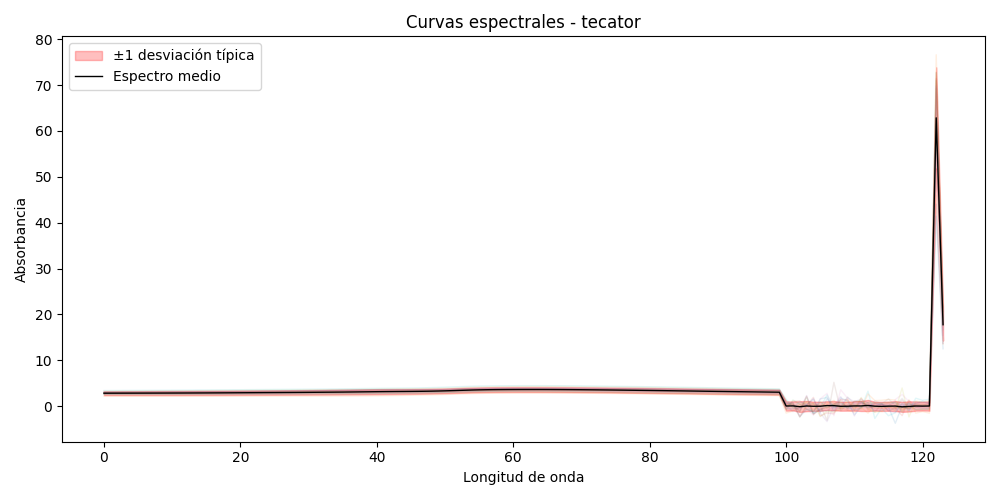
\includegraphics[width=0.7\linewidth]{../results/tecator/eda/eda_tecator_spectra.png}
    \caption{Espectros NIR del conjunto de datos Tecator.}
    \label{fig:tecator_spectra}
\end{figure}

La similitud entre espectros evidencia una estructura altamente correlacionada, donde las longitudes de onda adyacentes contienen información redundante. Este comportamiento sugiere la existencia de multicolinealidad severa y justifica el uso de técnicas basadas en reducción de dimensionalidad y extracción de componentes latentes.

Para analizar de forma más explícita la dependencia entre predictores, la Figura \ref{fig:tecator_corr} presenta la matriz de correlaciones entre variables espectrales.

\begin{figure}[H]
    \centering
    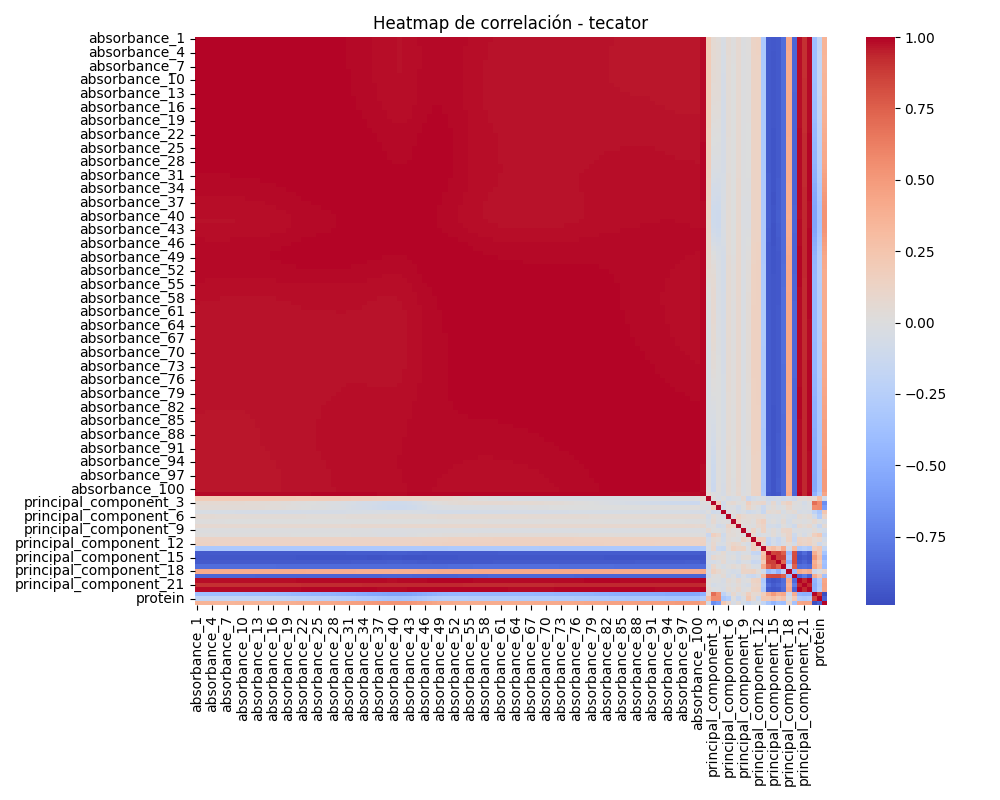
\includegraphics[width=0.60\linewidth]{../results/tecator/eda/eda_tecator_corr_heatmap.png}
    \caption{Mapa de correlaciones entre variables espectrales en Tecator.}
    \label{fig:tecator_corr}
\end{figure}

Se observan bloques extensos de correlaciones elevadas entre variables próximas, esto nos hace confirmar de manera empírica la presencia de multicolinealidad. Esto implica que la matriz $X^\top X$ se encuentra mal condicionada afectando negativamente la estabilidad de los coeficientes estimados mediante OLS.

La Figura \ref{fig:tecator_scree} muestra la proporción de varianza explicada acumulada por las componentes principales obtenidas mediante PCA.

\begin{figure}[!htbp]
    \centering
    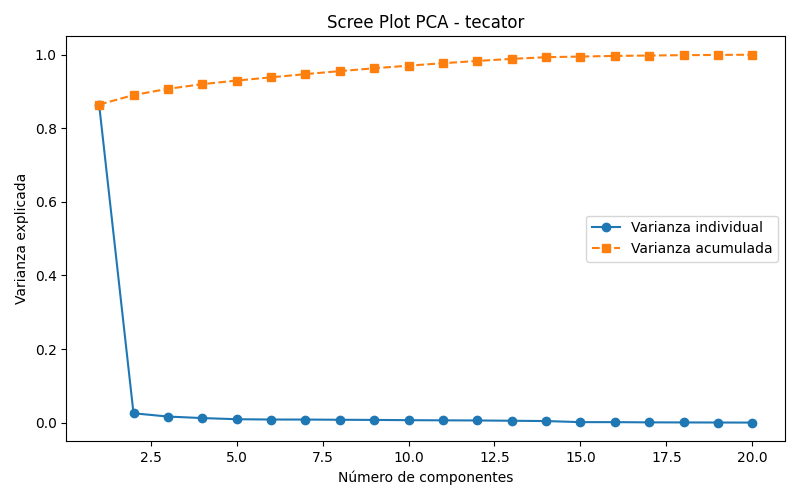
\includegraphics[width=0.60\linewidth]{../results/tecator/eda/eda_tecator_pca_scree.png}
    \caption{Varianza explicada acumulada mediante PCA en Tecator.}
    \label{fig:tecator_scree}
\end{figure}

Puede observarse que una proporción muy elevada de la variabilidad total queda explicada por las primeras componentes principales. Esto indica que la dimensionalidad efectiva del problema es considerablemente menor que el número original de variables, confirmando la existencia de una estructura latente de baja dimensión.

La representación de las observaciones sobre las primeras componentes principales se muestra en la Figura \ref{fig:tecator_scores}.

\begin{figure}[H]
    \centering
    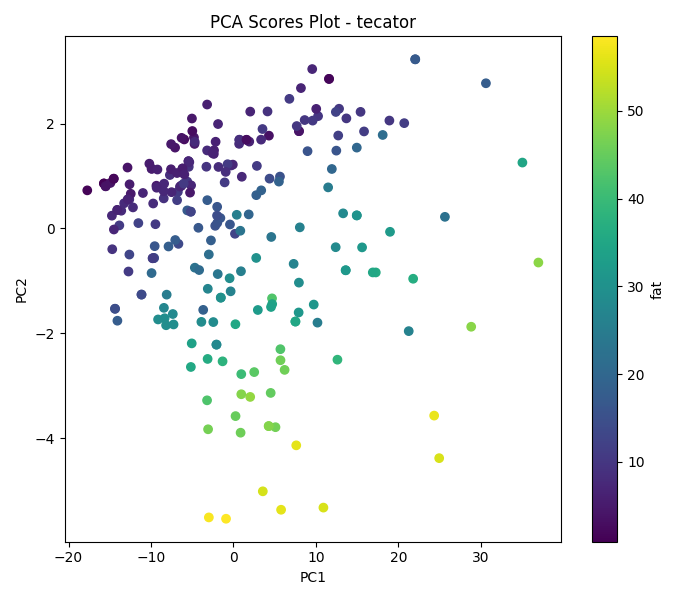
\includegraphics[width=0.60\linewidth]{../results/tecator/eda/eda_tecator_pca_scores.png}
    \caption{Representación de observaciones sobre las primeras componentes principales.}
    \label{fig:tecator_scores}
\end{figure}

Esta distribución sugiere una estructura continua y relativamente homogénea, sin agrupamientos extremos ni observaciones claramente atípicas, esto favorece el uso de modelos lineales basados en componentes latentes.

\subsection{Selección e interpretación del modelo PLS}

La selección del número óptimo de componentes en PLS se realizó mediante validación cruzada utilizando RMSE-CV como criterio principal. La evolución del error de validación se presenta en la Figura \ref{fig:pls_cv_tecator}.

\begin{figure}[!htbp]
    \centering
    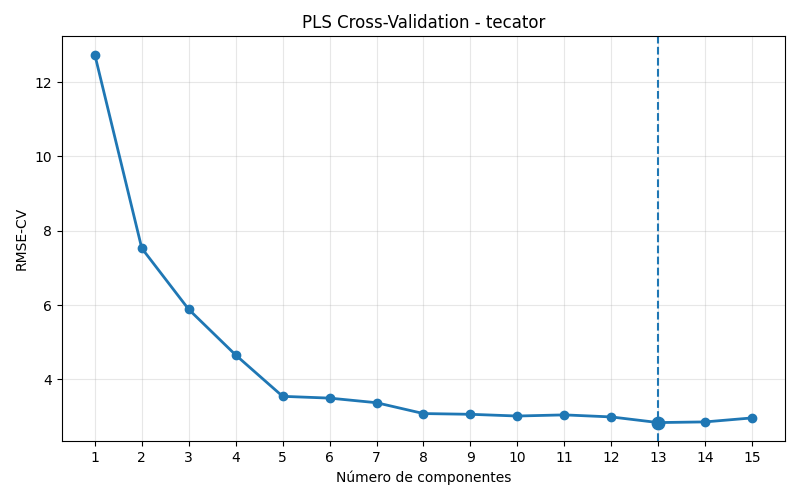
\includegraphics[width=0.75\linewidth]{../results/tecator/figures/pls_cv_tecator.png}
    \caption{RMSE-CV en función del número de componentes PLS en Tecator.}
    \label{fig:pls_cv_tecator}
\end{figure}

El modelo final se construyó utilizando 13 componentes latentes, ya que este valor corresponde al punto donde el RMSE-CV alcanza su mínimo y comienza posteriormente a estabilizarse. Este comportamiento indica que las primeras componentes capturan la mayor parte de la estructura predictiva presente en los datos, mientras que incrementar adicionalmente la complejidad del modelo aporta mejoras marginales en capacidad predictiva y puede comprometer su capacidad de generalización.

En la Figura \ref{fig:pls_loadings} se muestra que los loadings asociados a la primera componente presentan una estructura suave y continua a lo largo del espectro, comportamiento coherente con la naturaleza altamente correlacionada de los datos NIR.

\begin{figure}[!htbp]
    \centering
    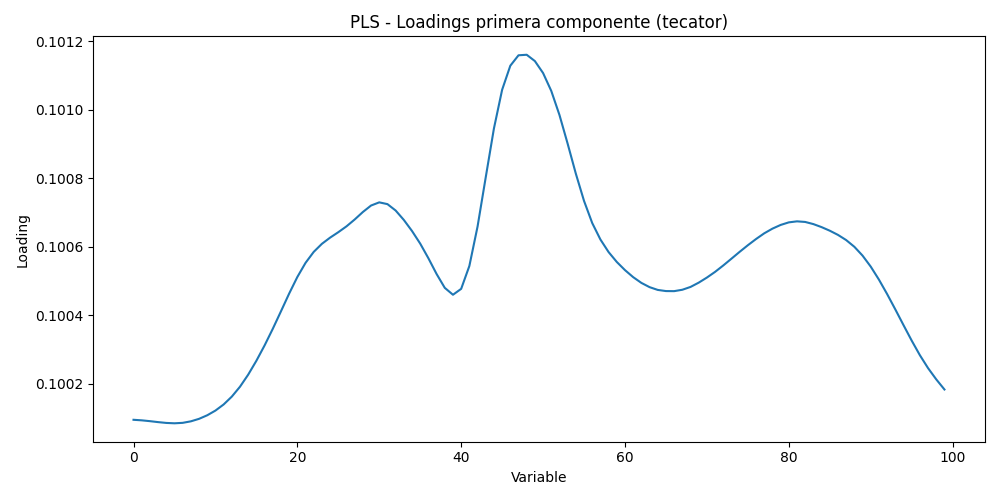
\includegraphics[width=0.85\linewidth]{../results/tecator/figures/pls_loadings.png}
    \caption{Loadings de las principales componentes PLS en Tecator.}
    \label{fig:pls_loadings}
\end{figure}

Se observan además regiones espectrales con contribuciones más pronunciadas (zona central), indicando que determinadas bandas espectrales poseen una mayor influencia en la construcción de la componente latente. Este comportamiento sugiere que la información predictiva relevante no se encuentra concentrada en variables aisladas, sino distribuida de forma continua entre regiones espectrales correlacionadas.

La ausencia de oscilaciones abruptas o patrones erráticos indica además que la componente extraída captura estructuras sistemáticas presentes en los datos y no fluctuaciones aleatorias asociadas al ruido.

\subsection{Comparación predictiva entre modelos}

El rendimiento predictivo de los distintos modelos evaluados sobre Tecator se resumen en la Tabla \ref{tab:tecator_results}.

\begin{table}[H]
\centering
\small
\caption{Comparación predictiva de modelos sobre Tecator.}
\label{tab:tecator_results}
\begin{tabular}{|c|c|c|c|c|}
\hline
\textbf{Modelo} & \textbf{RMSE} & \textbf{MAE} & \textbf{$R^2$} & \textbf{Adj-$R^2$} \\
\hline \hline
OLS    & 2.196 & 1.528 & 0.977 & 0.977 \\ \hline
PLS    & 2.789 & 1.991 & 0.964 & 0.963 \\ \hline
PCR    & 2.899 & 2.161 & 0.961 & 0.960 \\ \hline
Lasso  & 3.669 & 3.046 & 0.937 & 0.936 \\ \hline
Ridge  & 3.756 & 3.233 & 0.934 & 0.933 \\ \hline
\end{tabular}
\end{table}

Los resultados muestran que el modelo OLS obtiene el mejor rendimiento predictivo sobre el dataset Tecator, alcanzando el menor RMSE y el mayor coeficiente de determinación. Con esto podemos que observar que aunque el problema presenta multicolinealidad significativa, la dimensionalidad de Tecator sigue siendo moderada respecto al tamaño muestral ($n=215$, $p=100$), permitiendo que el estimador clásico mantenga una elevada capacidad predictiva.

Las métricas MAE y $R^2$ muestran un comportamiento consistente con los resultados observados mediante RMSE. OLS presenta simultáneamente el menor error absoluto medio y el mayor coeficiente de determinación, confirmando su superior capacidad predictiva sobre este conjunto de datos. PLS y PCR mantienen valores elevados de $R^2$, indicando que ambos modelos continúan capturando una proporción importante de la variabilidad presente en la variable respuesta.

PLS y PCR muestran un rendimiento competitivo, aunque ligeramente inferior al obtenido mediante OLS. A pesar que la reducción de dimensionalidad permite estabilizar la estimación y concentrar la información relevante en un número reducido de componentes, esto resultados sugieren que dicha compresión también puede descartar parte de la señal predictiva contenida en las variables originales. 

Estos resultados sugieren que las ventajas teóricas de PLS dependen fuertemente de la relación entre dimensionalidad, tamaño muestral y complejidad efectiva de la estructura latente. En escenarios donde el número de predictores no supera ampliamente al número de observaciones, la pérdida parcial de información derivada de la compresión en componentes puede superar los beneficios asociados a la reducción de varianza.

Desde el punto de vista estadístico, este comportamiento refleja el compromiso clásico entre sesgo y varianza. Mientras OLS minimiza el sesgo utilizando directamente todas las variables originales, métodos como PCR y PLS reducen la varianza mediante compresión dimensional, introduciendo simultáneamente un sesgo adicional asociado a la pérdida parcial de información predictiva.

En este caso, la estructura latente no resulta suficientemente compleja como para compensar completamente el sesgo introducido por la compresión de componentes y además el tamaño muestral relativamente elevado respecto al número de predictores permite que OLS conserve una excelente capacidad predictiva a pesar de la multicolinealidad existente.

PCR presenta un comportamiento ligeramente inferior a PLS, resultado coherente con la construcción supervisada de las componentes latentes en PLS. PCR maximiza exclusivamente la varianza explicada en $X$ y PLS incorpora información de la variable respuesta durante la extracción de componentes, favoreciendo direcciones predictivamente más relevantes.

Por otro lado, Ridge y Lasso presentan el peor comportamiento global. Aunque ambos métodos estabilizan la estimación mediante regularización, la penalización introducida genera una contracción excesiva de coeficientes en un escenario donde OLS todavía conserva estabilidad suficiente. Lasso particularmente produce soluciones más dispersas que pueden eliminar información útil distribuida en múltiples variables espectrales altamente correlacionadas.

La representación gráfica de la Figura \ref{fig:rmse_tecator} confirma los resultados observados previamente en la Tabla \ref{tab:tecator_results}.

\begin{figure}[H]
    \centering
    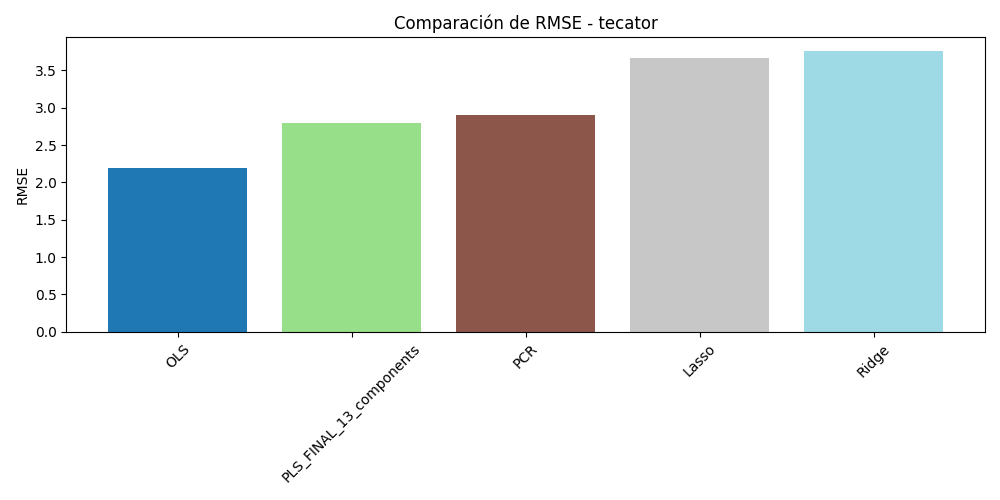
\includegraphics[width=0.60\linewidth]{../results/tecator/figures/rmse_tecator.png}
    \caption{Comparación del RMSE entre modelos en Tecator.}
    \label{fig:rmse_tecator}
\end{figure}

La Figura \ref{fig:comparison_pred_obs} compara la relación entre valores observados y predichos para los modelos OLS y PLS.

\begin{figure}[!htbp]
    \centering

    \begin{subfigure}[b]{0.48\textwidth}
        \centering
        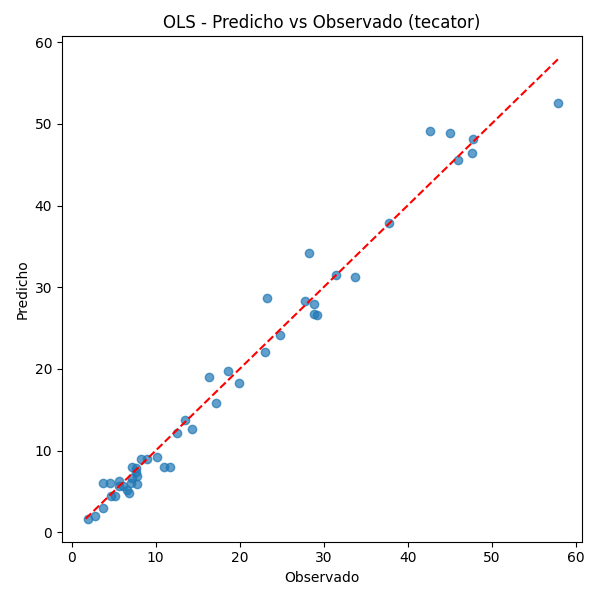
\includegraphics[width=\linewidth]{../results/tecator/figures/ols_pred_vs_obs.png}
        \caption{Modelo OLS}
        \label{fig:ols_pred_obs}
    \end{subfigure}
    \hfill
    \begin{subfigure}[b]{0.48\textwidth}
        \centering
        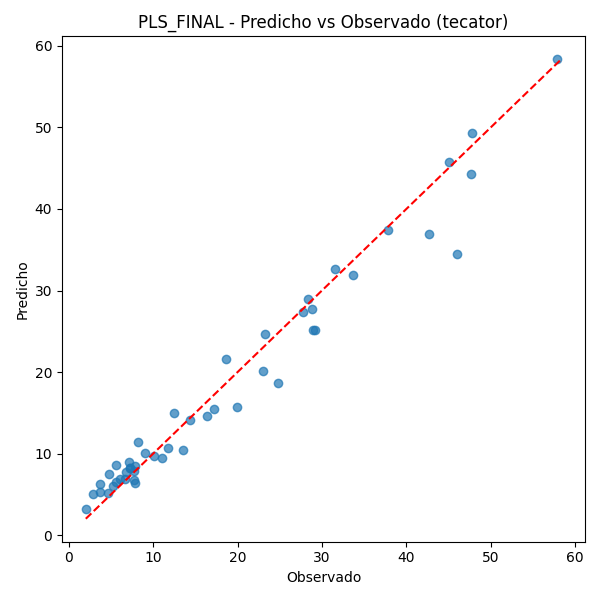
\includegraphics[width=\linewidth]{../results/tecator/figures/pls_pred_vs_obs.png}
        \caption{Modelo PLS}
        \label{fig:pls_pred_obs}
    \end{subfigure}

    \caption{Comparación entre valores observados y predichos para los modelos OLS y PLS en el dataset Tecator.}
    \label{fig:comparison_pred_obs}
\end{figure}

Ambos modelos muestran una elevada concordancia entre valores reales y estimados, observándose una concentración importante de observaciones alrededor de la diagonal identidad. Esto confirma que tanto OLS como PLS son capaces de capturar adecuadamente la relación existente entre los espectros NIR y el contenido graso.

Sin embargo, el modelo OLS presenta una alineación ligeramente más ajustada respecto a la diagonal, coherente con el menor RMSE observado previamente. Este comportamiento sugiere que el uso directo de todas las variables originales permite conservar información predictiva que puede perderse parcialmente durante la compresión en componentes latentes realizada por PLS.

PLS mantiene una elevada estabilidad predictiva y un comportamiento visualmente robusto, lo que confirma su capacidad para capturar la estructura latente subyacente incluso en presencia de fuerte multicolinealidad.

\subsection{Discusión de resultados}

Los resultados obtenidos sobre Tecator muestran que el comportamiento relativo de los modelos depende no solo de la presencia de multicolinealidad, sino también de la relación entre dimensionalidad, tamaño muestral y complejidad de la estructura latente subyacente.

Aunque el conjunto de datos presenta una fuerte correlación entre predictores y una estructura latente clara, el tamaño muestral sigue siendo suficientemente grande respecto al número de variables como para que OLS mantenga una elevada capacidad predictiva.

PLS y PCR logran capturar adecuadamente la estructura espectral mediante un número reducido de componentes latentes, mostrando un rendimiento competitivo y estable. Sin embargo, la reducción de dimensionalidad introduce un compromiso entre estabilización y pérdida parcial de información predictiva explicando su ligera inferioridad respecto a OLS en este escenario concreto.

Por otro lado, los resultados obtenidos por Ridge y Lasso sugieren que una regularización excesiva puede deteriorar el rendimiento cuando la señal predictiva se encuentra distribuida de forma continua entre múltiples variables altamente correlacionadas.

Tecator representa un escenario donde las ventajas teóricas de los métodos basados en componentes latentes son evidentes desde el punto de vista estructural e interpretativo, aunque no suficientemente pronunciadas como para superar el rendimiento predictivo del modelo clásico.

No obstante, los resultados obtenidos deben interpretarse dentro del contexto específico del conjunto de datos analizado. Las conclusiones pueden verse afectadas por la relación entre dimensionalidad y tamaño muestral, así como por la naturaleza aproximadamente lineal de la relación entre espectros y contenido graso. En escenarios con estructuras no lineales más complejas o con dimensionalidad extrema ($p \gg n$), el comportamiento relativo de los modelos podría diferir significativamente.

\section{Resultados en Gasoline}

El conjunto de datos Gasoline también representa un problema clásico de regresión espectral en quimiometría, caracterizado por una alta dimensionalidad y una fuerte correlación entre variables espectrales. Cada observación corresponde a un espectro NIR registrado en 401 longitudes de onda, mientras que la variable respuesta representa el índice de octanaje de la gasolina.

Estadísticamente, Gasoline constituye un escenario más complejo que Tecator, ya que el número de predictores supera ampliamente al número de observaciones ($p = 401$, $n = 60$). Esta situación genera una matriz de diseño altamente redundante y prácticamente singular, lo que dificulta la aplicación de métodos clásicos basados en mínimos cuadrados ordinarios y pudiendo favorecer el uso de técnicas de regularización y reducción supervisada de dimensionalidad.

\subsection{Análisis exploratorio y estructura latente}

La Figura \ref{fig:gasoline_spectra} muestra los espectros NIR correspondientes al conjunto Gasoline.

\begin{figure}[!htbp]
    \centering
    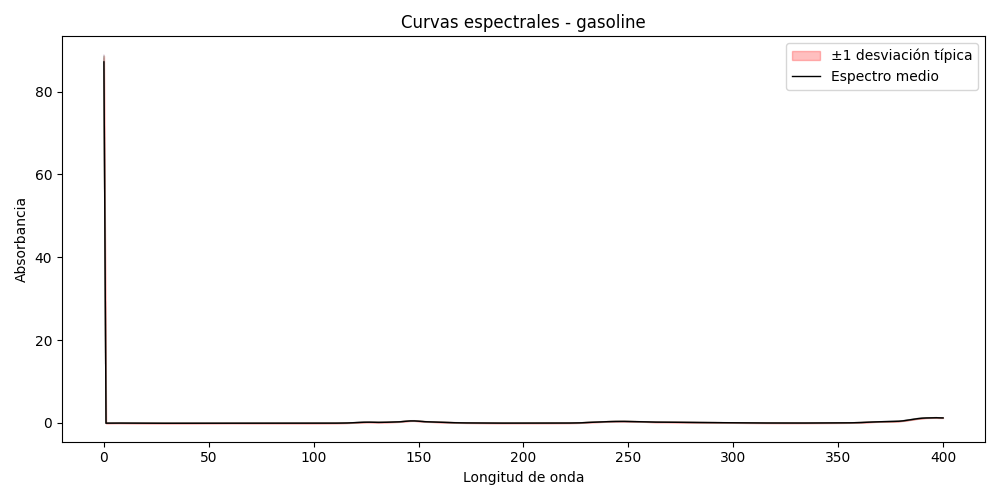
\includegraphics[width=0.8\textwidth]{../results/gasoline/eda/eda_gasoline_spectra.png}
    \caption{Espectros NIR del conjunto de datos Gasoline.}
    \label{fig:gasoline_spectra}
\end{figure}

Se observa nuevamente un comportamiento suave y continuo característico de datos espectrales NIR. La elevada similitud entre curvas evidencia una fuerte dependencia entre variables adyacentes y sugiere la presencia de multicolinealidad severa. Este comportamiento es típico en aplicaciones quimiométricas, donde múltiples longitudes de onda contienen información redundante sobre las propiedades químicas de la mezcla.

Con el objetivo de analizar la estructura latente presente en los datos, se aplicó un análisis de componentes principales (PCA). La Figura \ref{fig:gasoline_pca_scree} presenta la proporción de varianza explicada acumulada por las componentes principales.

\begin{figure}[!htbp]
    \centering
    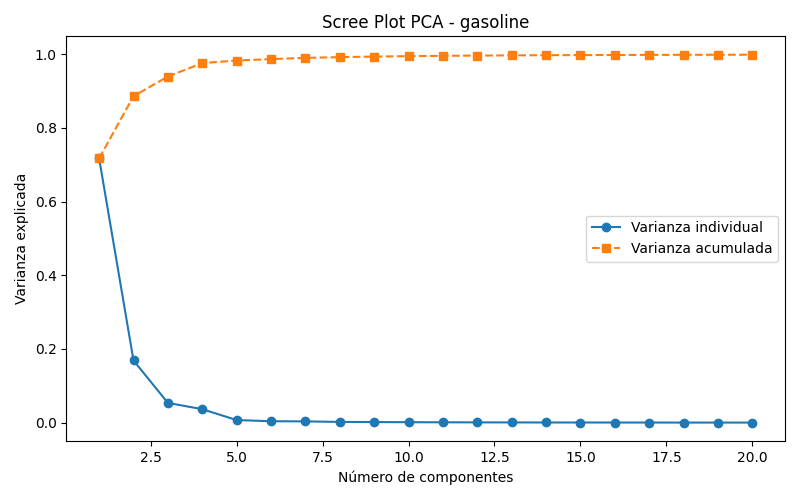
\includegraphics[width=0.75\textwidth]{../results/gasoline/eda/eda_gasoline_pca_scree.png}
    \caption{Varianza explicada acumulada mediante PCA en Gasoline.}
    \label{fig:gasoline_pca_scree}
\end{figure}

Puede observarse que las primeras componentes principales explican una proporción muy elevada de la variabilidad total, indicando que la dimensionalidad efectiva del problema es considerablemente menor que el número original de variables. Este comportamiento confirma la existencia de una estructura latente de baja dimensión, a pesar de la elevada dimensionalidad original del conjunto de datos.

La distribución observada en la Figura \ref{fig:gasoline_pca_scores} presenta una estructura relativamente dispersa, sin evidencia de agrupamientos completamente separados ni patrones claramente disjuntos. Este comportamiento sugiere la existencia de una estructura latente subyacente que puede representarse mediante un número reducido de direcciones principales, aunque posiblemente con una variabilidad más heterogénea que la observada previamente en Tecator.

\begin{figure}[!htbp]
    \centering
    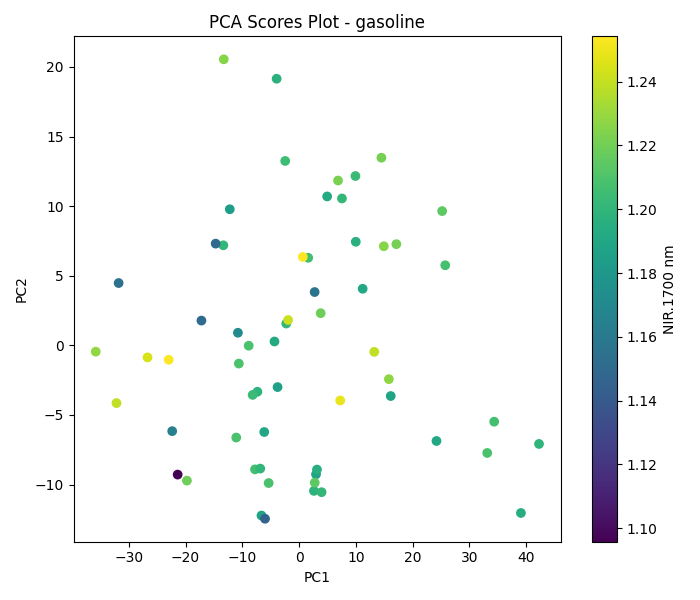
\includegraphics[width=0.75\textwidth]{../results/gasoline/eda/eda_gasoline_pca_scores.png}
    \caption{Representación de observaciones sobre las primeras componentes principales en Gasoline.}
    \label{fig:gasoline_pca_scores}
\end{figure}

La dispersión observada resulta coherente con la mayor complejidad estructural del dataset Gasoline y con la presencia simultánea de alta dimensionalidad y fuerte correlación entre variables espectrales. Este tipo de estructura favorece el uso de modelos lineales basados en componentes latentes y técnicas de regularización capaces de estabilizar la estimación en presencia de multicolinealidad severa.

\subsection{Selección e interpretación del modelo PLS}

La selección del número óptimo de componentes en PLS se realizó mediante validación cruzada utilizando RMSE-CV como criterio principal. La evolución del error de validación se presenta en la Figura \ref{fig:gasoline_pls_cv}.

\begin{figure}[!htbp]
    \centering
    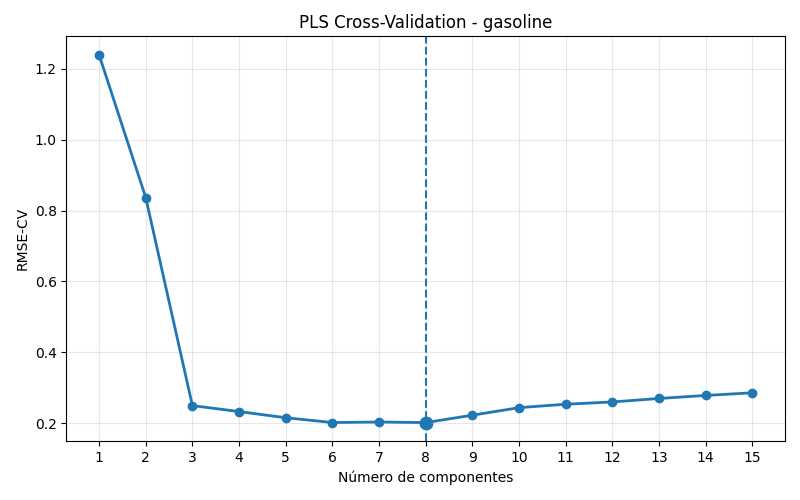
\includegraphics[width=0.75\textwidth]{../results/gasoline/figures/pls_cv_gasoline.png}
    \caption{RMSE-CV en función del número de componentes PLS en Gasoline.}
    \label{fig:gasoline_pls_cv}
\end{figure}

El modelo final se construyó utilizando el número de componentes correspondiente al mínimo de RMSE-CV. Se observa que el error disminuye rápidamente durante las primeras componentes y posteriormente comienza a estabilizarse, indicando que la mayor parte de la estructura predictiva relevante queda capturada en un número relativamente reducido de componentes latentes.

La Figura \ref{fig:gasoline_pls_loadings} muestra los loadings asociados a la primera componente PLS en Gasoline. Aquí aparecen regiones espectrales con cambios más marcados de signo y variaciones de mayor amplitud, especialmente en determinados intervalos del espectro. Este comportamiento sugiere que la contribución de las variables espectrales a la construcción de la componente latente no es homogénea, sino que ciertas bandas específicas poseen una influencia considerablemente mayor sobre la predicción del índice de octanaje.

\begin{figure}[!htbp]
    \centering
    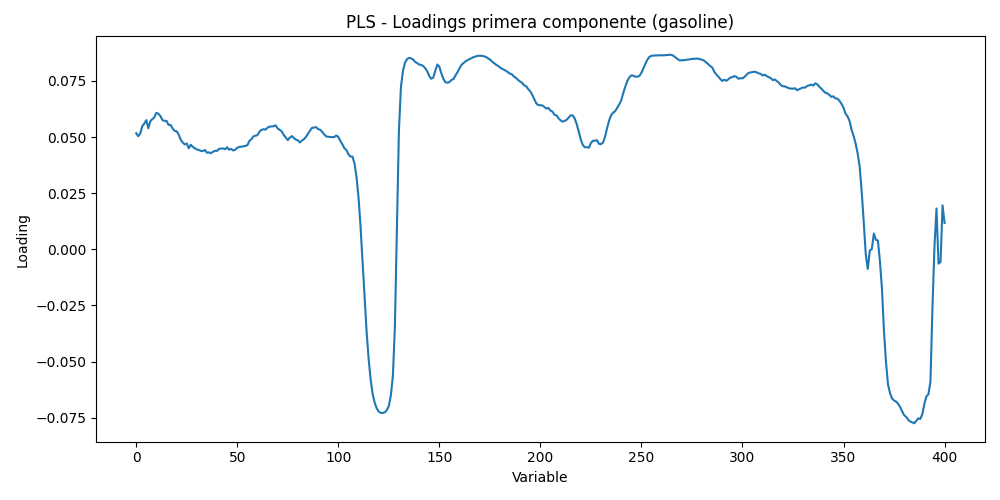
\includegraphics[width=0.75\textwidth]{../results/gasoline/figures/pls_loadings.png}
    \caption{Loadings de las principales componentes PLS en Gasoline.}
    \label{fig:gasoline_pls_loadings}
\end{figure}

Puede observarse además que amplias regiones del espectro mantienen loadings positivos relativamente estables, mientras que otras zonas presentan caídas pronunciadas hacia valores negativos. Esto nos indica que distintas regiones espectrales contribuyen de manera diferenciada e incluso opuesta a la construcción de la componente latente, reflejando una estructura predictiva más compleja que la observada previamente en Tecator.

La presencia de transiciones relativamente suaves entre regiones confirma además que la componente extraída captura patrones estructurales reales asociados a la señal espectral y no únicamente fluctuaciones aleatorias debidas al ruido. Este comportamiento resulta coherente con la naturaleza altamente correlacionada de los espectros NIR y con la existencia de relaciones latentes complejas entre las bandas espectrales y el índice de octanaje.


\subsection{Comparación predictiva entre modelos}

El rendimiento predictivo de los distintos modelos evaluados sobre Gasoline se resume en la Tabla \ref{tab:gasoline_results}.



\begin{table}[H]
\centering
\small
\caption{Comparación predictiva de modelos sobre Gasoline.}
\label{tab:gasoline_results}
\begin{tabular}{|c|c|c|c|c|}
\hline
\textbf{Modelo} & \textbf{RMSE} & \textbf{MAE} & \textbf{$R^2$} & \textbf{Adj-$R^2$} \\
\hline \hline
Lasso & 0.255 & 0.192 & 0.967 & 0.964 \\
PCR   & 0.295 & 0.238 & 0.956 & 0.951 \\
Ridge & 0.327 & 0.235 & 0.946 & 0.940 \\
OLS   & 0.345 & 0.252 & 0.940 & 0.933 \\
PLS   & 0.363 & 0.267 & 0.933 & 0.927 \\
\hline
\end{tabular}
\end{table}

Los resultados muestran que el modelo Lasso obtiene el mejor rendimiento predictivo sobre el conjunto de datos Gasoline, obteniendo simultáneamente el menor RMSE y el mayor coeficiente de determinación. Este comportamiento sugiere que la información predictiva relevante parece concentrarse principalmente en determinadas regiones espectrales específicas, aunque los datos presentan una fuerte estructura latente y elevada correlación entre predictores.

La penalización $L_1$ que Lasso introduce, ha favorecido la construcción de modelos más parsimoniosos mediante selección automática de variables, permitiendo identificar subconjuntos relevantes dentro de un espacio predictor altamente redundante. Este comportamiento resulta especialmente favorable en escenarios donde $p > n$, tal como es Gasoline.

En la Figura \ref{fig:gasoline_lasso_importance} puede observarse que únicamente un número reducido de variables presenta coeficientes de magnitud elevada, mientras que gran parte de las variables espectrales quedan fuertemente penalizadas o próximas a cero. Este comportamiento confirma empíricamente la capacidad de Lasso para inducir sparsity y seleccionar automáticamente regiones espectrales relevantes para la predicción del índice de octanaje.

\begin{figure}[!htbp]
    \centering
    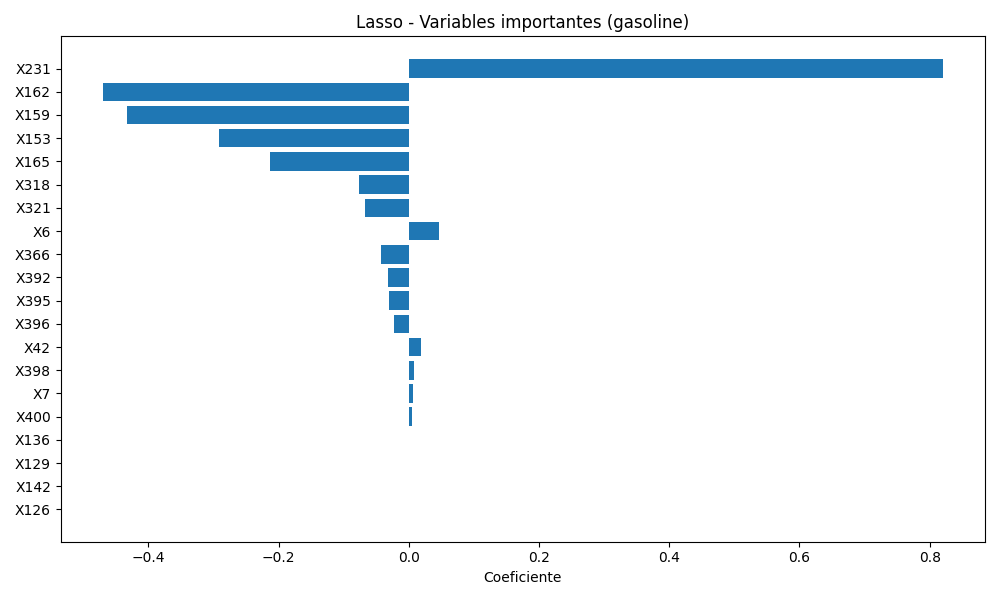
\includegraphics[width=0.6\textwidth]{../results/gasoline/figures/lasso_importance.png}
    \caption{Variables espectrales más relevantes seleccionadas por Lasso en Gasoline.}
    \label{fig:gasoline_lasso_importance}
\end{figure}

En la Figura \ref{fig:gasoline_rmse} se evidencia que que Lasso presenta el menor RMSE entre todos los modelos evaluados, seguido por PCR, Ridge, OLS y finalmente PLS. Las diferencias observadas reflejan cómo distintos enfoques de regularización y reducción de dimensionalidad responden ante un escenario caracterizado por alta dimensionalidad y fuerte multicolinealidad.

\begin{figure}[H]
    \centering
    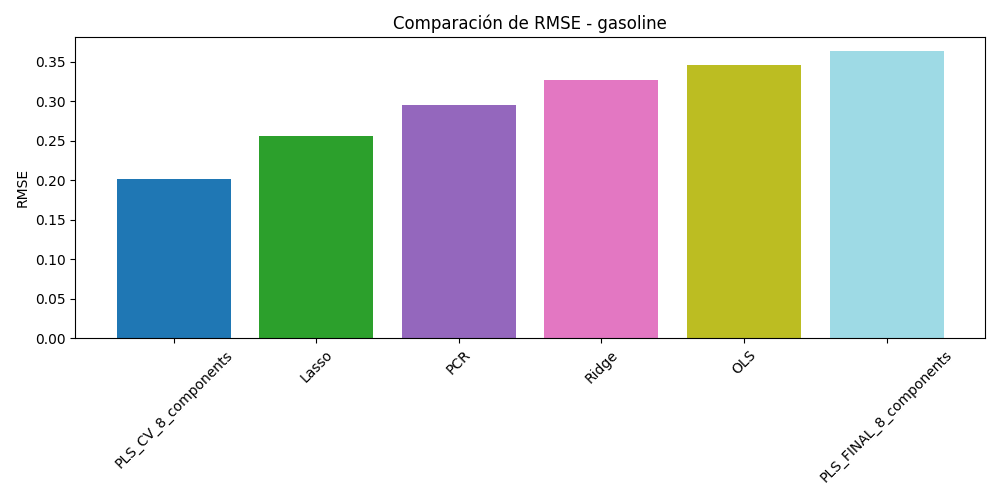
\includegraphics[width=0.6\textwidth]{../results/gasoline/figures/rmse_gasoline.png}
    \caption{Comparación del RMSE entre modelos en Gasoline.}
    \label{fig:gasoline_rmse}
\end{figure}

PCR muestra un comportamiento particularmente competitivo, obteniendo un RMSE relativamente cercano al alcanzado por Lasso. Este resultado confirma la existencia de una estructura latente de baja dimensionalidad en los espectros NIR, donde gran parte de la variabilidad relevante puede representarse mediante un número reducido de componentes principales.

Ridge y OLS mantienen también un rendimiento estable, conservando valores elevados de $R^2$ y errores predictivos relativamente reducidos. Lo que nos dice que la relación entre los espectros NIR y el índice de octanaje mantiene una estructura aproximadamente lineal y estable incluso en presencia de elevada dimensionalidad y fuerte multicolinealidad.

PLS presenta el mayor RMSE entre los modelos evaluados, sin embargo mantiene todavía un rendimiento predictivo razonablemente competitivo. El comportamiento relativamente competitivo de OLS debe interpretarse con cautela, ya que en este escenario \(p > n\) la solución obtenida corresponde a una estimación basada en pseudoinversa y no al estimador clásico de mínimos cuadrados ordinarios.Con esto observamos que la compresión supervisada mediante componentes latentes no logra explotar la estructura predictiva de forma tan eficiente como los enfoques basados en selección automática de variables o reducción no supervisada de dimensionalidad.

Al comparar la relacion entre valores observados y predichos para los modelos Lasso y PLS tal como vemos en la Figura \ref{fig:gasoline_obs_pred} se puede detallar una elevada concordancia entre valores observados y predichos, observándose una concentración importante de observaciones alrededor de la diagonal identidad. Esto confirma que tanto Lasso como PLS son capaces de capturar adecuadamente la relación existente entre los espectros NIR y el índice de octanaje.

\begin{figure}[H]
    \centering
    \begin{subfigure}{0.48\textwidth}
        \centering
        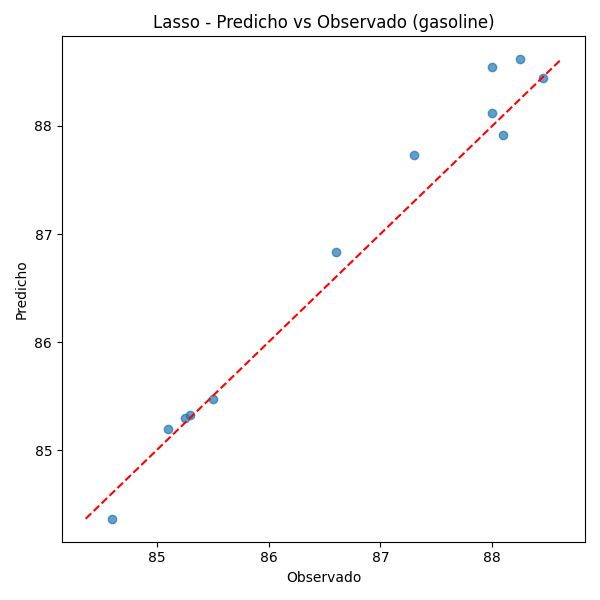
\includegraphics[width=\textwidth]{../results/gasoline/figures/lasso_pred_vs_obs.png}
        \caption{Modelo Lasso}
    \end{subfigure}
    \hfill
    \begin{subfigure}{0.48\textwidth}
        \centering
        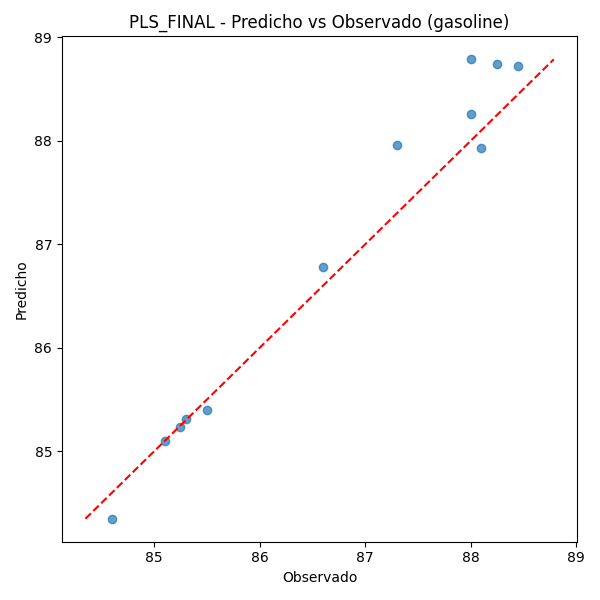
\includegraphics[width=\textwidth]{../results/gasoline/figures/pls_pred_vs_obs.png}
        \caption{Modelo PLS}
    \end{subfigure}
    \caption{Comparación entre valores observados y predichos para los modelos Lasso y PLS en Gasoline.}
    \label{fig:gasoline_obs_pred}
\end{figure}

Sin embargo, el modelo Lasso presenta una alineación ligeramente más ajustada respecto a la diagonal, que concuerda con el menor RMSE observado previamente. La dispersión de los errores resulta también ligeramente menor en comparación con PLS, indicando una mejor capacidad de generalización sobre este conjunto de datos.

PLS mantiene igualmente un comportamiento estable y robusto, confirmando su capacidad para capturar la estructura latente subyacente incluso en presencia de multicolinealidad severa y alta dimensionalidad. De igual manera, los resultados sugieren que en este escenario concreto la selección automática de variables realizada por Lasso permite explotar de forma más eficiente la estructura predictiva presente en determinadas regiones espectrales.

\subsection{Discusión de resultados}

Los resultados obtenidos sobre Gasoline muestran un comportamiento claramente distinto al observado previamente en Tecator. Aunque ambos conjuntos de datos corresponden a problemas espectrales con fuerte multicolinealidad y estructura latente, la relación $p > n$ presente en Gasoline genera un escenario considerablemente más favorable para métodos basados en regularización.

Es por ello que Lasso obtiene el mejor rendimiento predictivo global, evidenciando cómo la selección automática de variables puede resultar especialmente efectiva cuando la información relevante se encuentra parcialmente concentrada en determinadas regiones espectrales. La capacidad del modelo para inducir sparsity permite reducir redundancia y mejorar la estabilidad predictiva en un problema de elevada dimensionalidad.

PCR presenta igualmente un comportamiento altamente competitivo, confirmando la existencia de una estructura latente de baja dimensionalidad en los espectros NIR. Este resultado indica que gran parte de la variabilidad relevante puede representarse adecuadamente mediante un número reducido de componentes principales.

Aunque PLS logra capturar correctamente la relación entre variables espectrales y respuesta, su rendimiento predictivo resulta ligeramente inferior al obtenido mediante Lasso y PCR. Esto nos muestra que para este conjunto de datos, la compresión supervisada en componentes latentes no consigue explotar la estructura predictiva con la misma eficacia que los enfoques basados en selección de variables o reducción no supervisada de dimensionalidad.

\section{Resultados en Riboflavin}

El conjunto de datos Riboflavin está representando un escenario extremo de alta dimensionalidad en bioinformática, caracterizado por la presencia simultánea de multicolinealidad severa, sparsity y una relación $p \gg n$. Cada observación corresponde a niveles de expresión génica en \textit{Bacillus subtilis}, registrados para 4088 genes, mientras que la variable respuesta representa la producción de riboflavina.

A modo estadístico, este dataset presenta un problema más complejo que los analizados previamente en Tecator y Gasoline. El número de predictores supera ampliamente al número de observaciones ($p = 4088$, $n = 71$), generando una matriz de diseño altamente redundante y singular. Teóricamente en estos escenarios, los métodos clásicos basados en OLS tienden a presentar elevada inestabilidad y riesgo de sobreajuste, favoreciendo el uso de técnicas de regularización y reducción supervisada de dimensionalidad.

\subsection{Análisis exploratorio y estructura latente}

En la Figura \ref{fig:riboflavin_variance} puede observarse la distribución de la varianza de los niveles de expresión génica. Se aprecia una elevada heterogeneidad entre genes, donde una gran proporción presenta varianza reducida mientras que únicamente un subconjunto pequeño exhibe variabilidad considerablemente mayor.

\begin{figure}[!htbp]
    \centering
    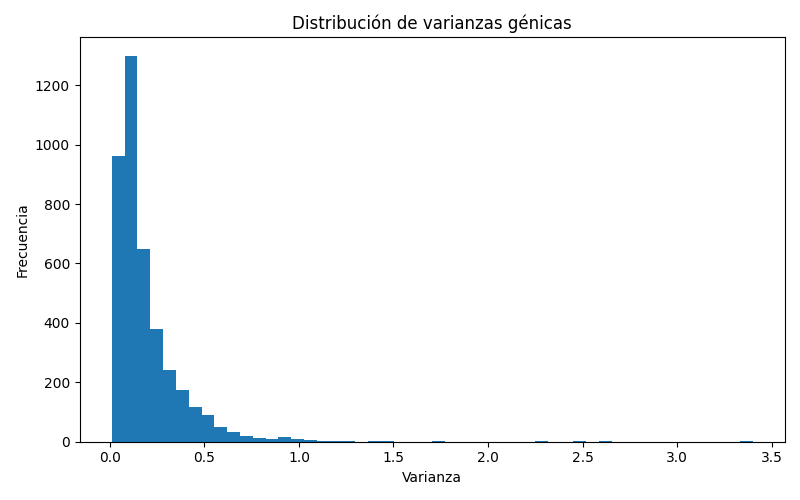
\includegraphics[width=0.6\textwidth]{../results/riboflavin/eda/eda_riboflavin_variance_hist.png}
    \caption{Distribución de varianza en Riboflavin.}
    \label{fig:riboflavin_variance}
\end{figure}

Para analizar la estructura latente presente en los datos, se aplicó un análisis de componentes principales (PCA). La Figura \ref{fig:riboflavin_pca_scree} muestra la proporción de varianza explicada acumulada por las componentes principales.

\begin{figure}[!htbp]
    \centering
    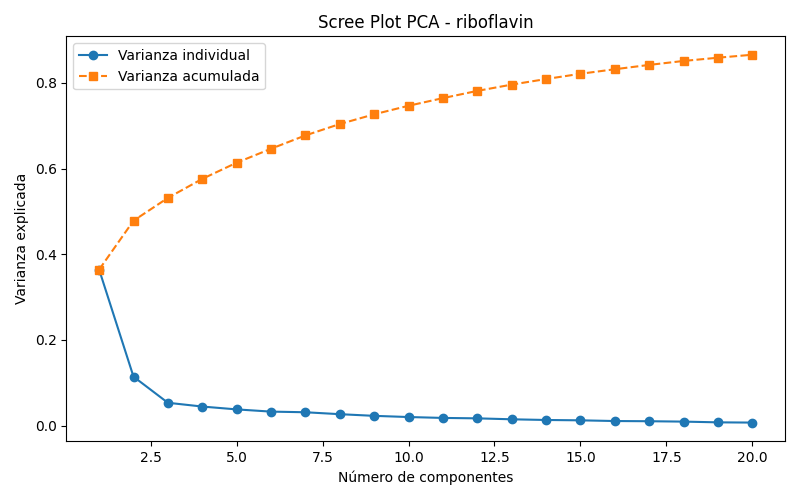
\includegraphics[width=0.6\textwidth]{../results/riboflavin/eda/eda_riboflavin_pca_scree.png}
    \caption{Varianza explicada acumulada mediante PCA en Riboflavin.}
    \label{fig:riboflavin_pca_scree}
\end{figure}

Puede observarse que las primeras componentes principales capturan una proporción importante de la variabilidad total, aunque la convergencia hacia valores elevados de varianza explicada resulta más gradual que en los datasets espectrales analizados previamente. Esto nos indica que la estructura latente en Riboflavin es considerablemente más compleja y dispersa, con información relevante distribuida entre múltiples direcciones del espacio predictor.

La representación de las observaciones sobre las primeras componentes principales se presenta en la Figura \ref{fig:riboflavin_pca_scores}, donde se observa una distribución relativamente dispersa y heterogénea, sin evidencia de agrupamientos claramente definidos ni patrones estructurales evidentes. Este comportamiento sugiere la presencia de relaciones latentes complejas y posiblemente no lineales, donde múltiples procesos biológicos pueden contribuir simultáneamente a la variabilidad observada en los niveles de expresión génica. 

\begin{figure}[H]
    \centering
    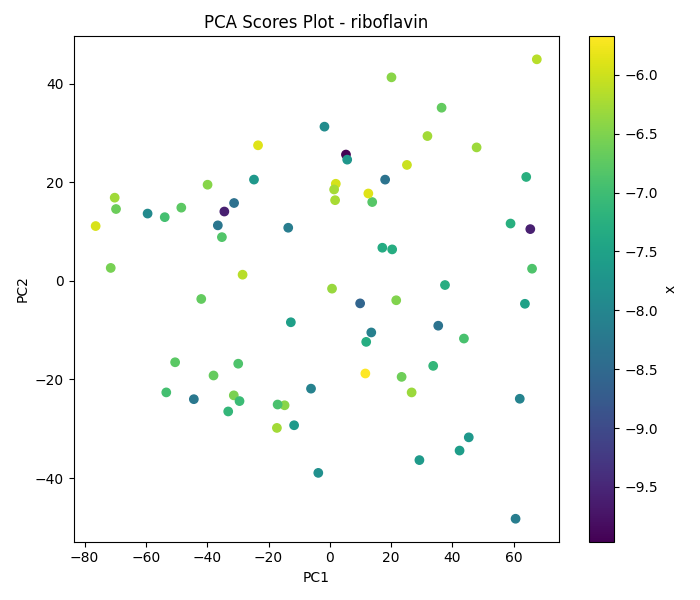
\includegraphics[width=0.6\textwidth]{../results/riboflavin/eda/eda_riboflavin_pca_scores.png}
    \caption{Representación de observaciones sobre las primeras componentes principales en Riboflavin.}
    \label{fig:riboflavin_pca_scores}
\end{figure}

Con el objetivo de explorar relaciones locales entre genes altamente variables, la Figura \ref{fig:riboflavin_heatmap} presenta un mapa de calor correspondiente a los genes más relevantes.

\begin{figure}[!htbp]
    \centering
    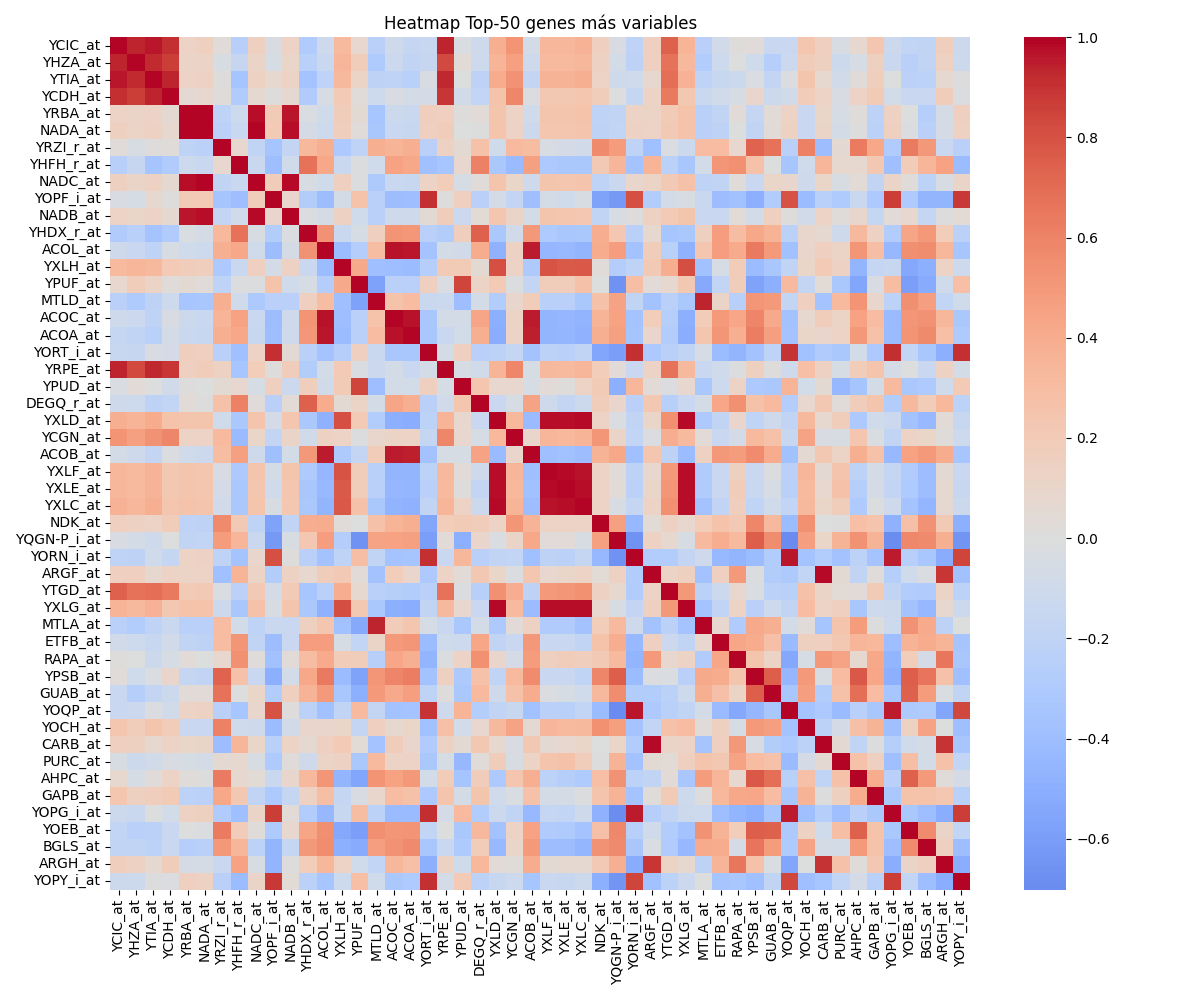
\includegraphics[width=0.6\textwidth]{../results/riboflavin/eda/eda_riboflavin_top_genes_heatmap.png}
    \caption{Mapa de correlaciones entre variables espectrales en Riboflavin.}
    \label{fig:riboflavin_heatmap}
\end{figure}

Se observan además bloques de genes con comportamientos similares entre muestras, indicando la presencia de patrones de coexpresión génica. Esto hace que determinados grupos de genes presenten dependencias estructurales y relaciones de correlación elevadas, confirmando la existencia de multicolinealidad extrema dentro del espacio predictor. Es por ello que debemos aplicar métodos capaces de estabilizar la estimación en presencia de esta complejidad estructural, como PLS o técnicas de regularización.

\subsection{Selección e interpretación del modelo PLS}

La selección del número óptimo de componentes en PLS se realizó mediante validación cruzada utilizando RMSE-CV como criterio principal. La evolución del error de validación se muestra en la Figura \ref{fig:riboflavin_pls_cv}.

\begin{figure}[!htbp]
    \centering
    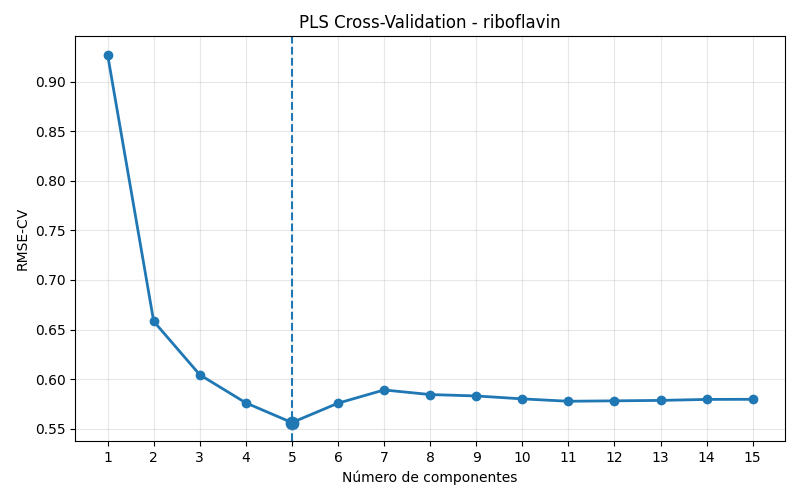
\includegraphics[width=0.7\textwidth]{../results/riboflavin/figures/pls_cv_riboflavin.png}
    \caption{RMSE-CV en función del número de componentes PLS en Riboflavin.}
    \label{fig:riboflavin_pls_cv}
\end{figure}

El error de validación disminuye rápidamente durante las primeras componentes y alcanza su mínimo utilizando 5 componentes latentes. A partir de allí la mejora predictiva se estabiliza, indicando que las primeras componentes capturan la mayor parte de la información relevante presente en los datos.

Este comportamiento resulta coherente con la naturaleza de los problemas de expresión génica, donde aunque el número de variables es extremadamente elevado, gran parte de la señal predictiva efectiva suele concentrarse en un subconjunto reducido de estructuras latentes asociadas a procesos biológicos subyacentes.

La reducción supervisada de dimensionalidad realizada por PLS permite estabilizar la estimación incluso en presencia de una matriz $X^\top X$ singular, evitando el sobreajuste asociado a la utilización directa de miles de predictores altamente correlacionados.

\subsection{Comparación predictiva entre modelos}

El rendimiento predictivo de los distintos modelos evaluados sobre Riboflavin se resume en la Tabla \ref{tab:riboflavin_results}.

\begin{table}[H]
\centering
\small
\caption{Comparación predictiva de modelos sobre Riboflavin.}
\label{tab:riboflavin_results}
\begin{tabular}{|c|c|c|c|c|}
\hline
\textbf{Modelo} & \textbf{RMSE} & \textbf{MAE} & \textbf{$R^2$} & \textbf{Adj-$R^2$} \\
\hline \hline
PLS    & 0.341 & 0.275 & 0.799 & 0.783 \\ \hline
Ridge  & 0.358 & 0.280 & 0.779 & 0.762 \\ \hline
OLS    & 0.358 & 0.280 & 0.779 & 0.762 \\ \hline
Lasso  & 0.443 & 0.390 & 0.661 & 0.635 \\ \hline
PCR    & 0.592 & 0.484 & 0.394 & 0.347 \\ \hline
\end{tabular}
\end{table}

Los resultados muestran que el modelo PLS obtiene el mejor rendimiento predictivo global sobre Riboflavin, alcanzando simultáneamente el menor RMSE y el mayor coeficiente de determinación. Este comportamiento resulta coherente con las propiedades teóricas de PLS en escenarios de alta dimensionalidad extrema y fuerte multicolinealidad.

La construcción supervisada de componentes latentes permite que PLS capture direcciones del espacio predictor altamente relacionadas con la variable respuesta, concentrando la información predictiva relevante en un número reducido de componentes. Esto favorece simultáneamente la reducción de varianza, la estabilidad numérica y la capacidad de generalización.

La Figura \ref{fig:riboflavin_rmse} confirma gráficamente las diferencias observadas previamente entre modelos. Ridge y OLS presentan un rendimiento relativamente competitivo y muy similar entre sí. El uso de regularización implícita y la estructura latente subyacente permiten que ambos métodos mantengan una capacidad predictiva razonablemente elevada. Sin embargo, sus resultados continúan siendo ligeramente inferiores a los obtenidos mediante PLS.

\begin{figure}[!htbp]
    \centering
    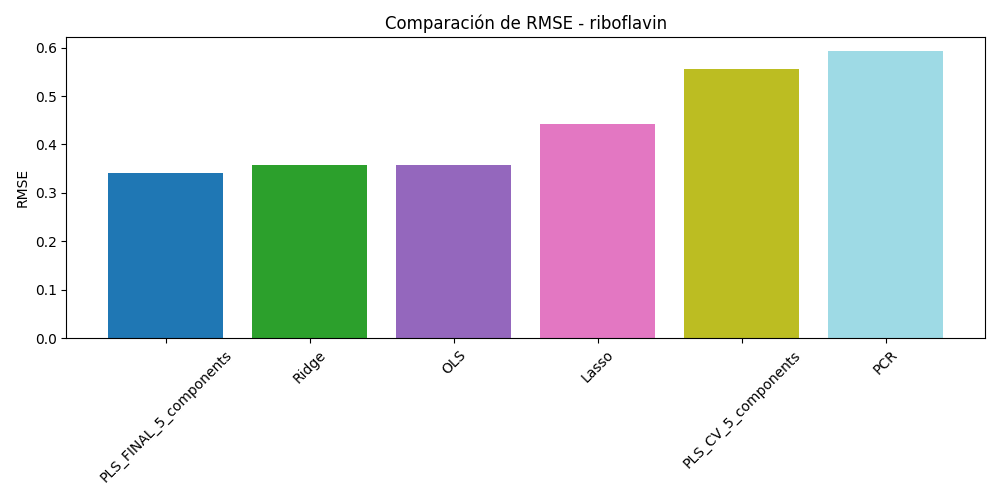
\includegraphics[width=0.75\textwidth]{../results/riboflavin/figures/rmse_riboflavin.png}
    \caption{Comparación del RMSE entre modelos en Riboflavin.}
    \label{fig:riboflavin_rmse}
\end{figure}

Lasso presenta un rendimiento moderadamente inferior, indicando que la información predictiva relevante probablemente no se encuentra concentrada únicamente en un subconjunto extremadamente reducido de genes aislados, sino distribuida de manera más continua entre múltiples grupos de variables correlacionadas. La penalización $L_1$ puede inducir entonces una selección excesivamente agresiva, eliminando parte de la señal útil.

PCR presenta el peor comportamiento global entre los modelos evaluados. Este resultado refleja una limitación clásica de los enfoques no supervisados de reducción de dimensionalidad. Al construir las componentes únicamente maximizando la varianza explicada en $X$, PCR puede descartar direcciones con baja varianza pero alta relevancia predictiva para la producción de riboflavin.

La Figura \ref{fig:riboflavin_obs_pred} compara la relación entre valores observados y predichos para los modelos OLS, Ridge y PLS.

\begin{figure}[!htbp]
    \centering

    \begin{subfigure}[b]{0.32\textwidth}
        \centering
        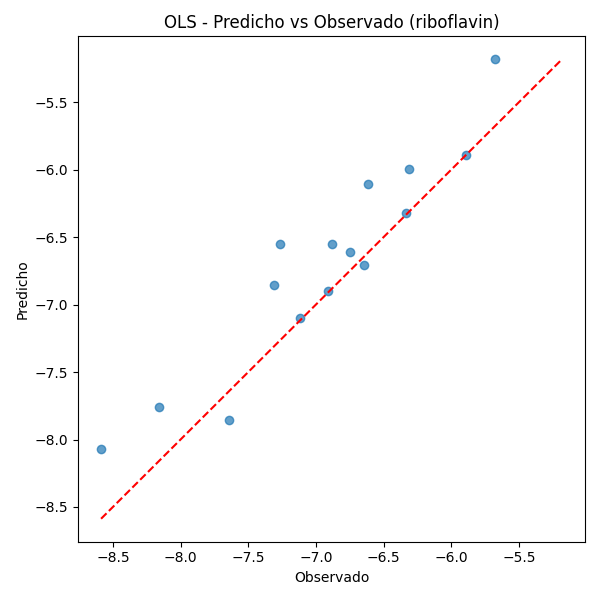
\includegraphics[width=\linewidth]{../results/riboflavin/figures/ols_pred_vs_obs.png}
        \caption{Modelo OLS}
    \end{subfigure}
    \hfill
    \begin{subfigure}[b]{0.32\textwidth}
        \centering
        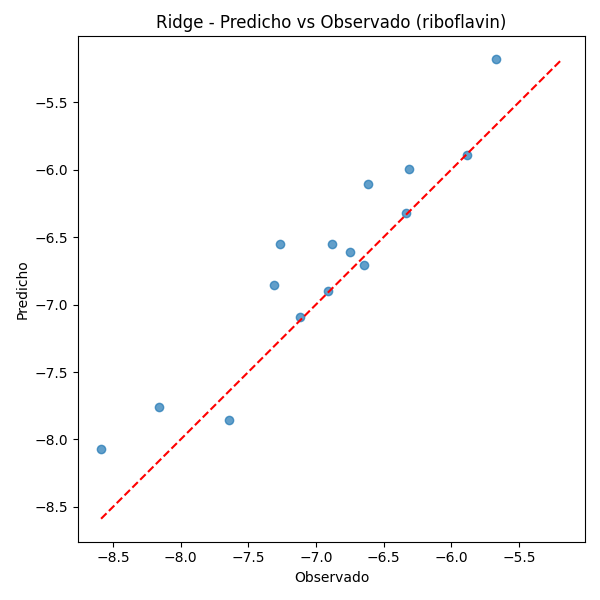
\includegraphics[width=\linewidth]{../results/riboflavin/figures/ridge_pred_vs_obs.png}
        \caption{Modelo Ridge}
    \end{subfigure}
    \hfill
    \begin{subfigure}[b]{0.32\textwidth}
        \centering
        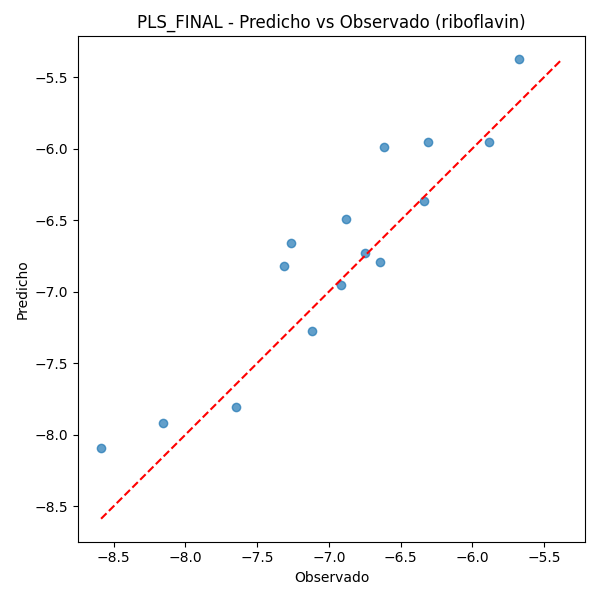
\includegraphics[width=\linewidth]{../results/riboflavin/figures/pls_pred_vs_obs.png}
        \caption{Modelo PLS}
    \end{subfigure}

    \caption{Comparación entre valores observados y predichos para los modelos OLS, Ridge y PLS en Riboflavin.}
    \label{fig:riboflavin_obs_pred}
\end{figure}

Los tres modelos muestran una relación aproximadamente lineal entre valores observados y predichos, indicando que todos son capaces de capturar parcialmente la estructura subyacente del problema. Sin embargo, PLS presenta una alineación más ajustada respecto a la diagonal identidad y una dispersión de errores ligeramente menor, lo que es coherente con el menor RMSE obtenido previamente. Este comportamiento puede indicarnos que la reducción supervisada de dimensionalidad implementada por PLS permite capturar de forma más eficiente la estructura latente compleja presente en los datos, mejorando la capacidad de generalización incluso en un escenario caracterizado por una relación $p \gg n$ y multicolinealidad extrema.

\subsection{Discusión de resultados}

Los resultados obtenidos sobre Riboflavin representan el escenario más favorable para métodos basados en reducción supervisada de dimensionalidad dentro de los conjuntos de datos analizados en este trabajo.

La combinación simultánea de alta dimensionalidad, fuerte correlación entre genes y complejidad estructural favorece claramente el uso de metodologías capaces de estabilizar la estimación y concentrar la información relevante en un número reducido de componentes.

PLS logra explotar eficientemente esta estructura mediante la construcción supervisada de componentes latentes orientadas hacia la covarianza entre predictores y respuesta, obteniendo el mejor rendimiento predictivo global. Este comportamiento resulta tal como la literatura sobre aplicaciones de PLS en bioinformática y datos genómicos, donde el método suele mostrar ventajas importantes frente a enfoques no supervisados.

Los resultados obtenidos por PCR muestran además que una reducción de dimensionalidad basada exclusivamente en la varianza explicada puede resultar insuficiente en problemas donde la información predictiva relevante no coincide necesariamente con las direcciones de mayor variabilidad global.

El comportamiento competitivo de Ridge y OLS sugiere que la relación entre expresión génica y producción de riboflavina mantiene una estructura aproximadamente lineal que puede capturarse parcialmente incluso mediante modelos clásicos. 

Los resultados obtenidos por OLS deben interpretarse con cautela. En escenarios de alta dimensionalidad extrema (\(p \gg n\)), la solución obtenida mediante pseudoinversa puede presentar elevada inestabilidad y sensibilidad al ruido, por lo que un buen rendimiento predictivo no implica necesariamente una estimación robusta o interpretable de los coeficientes.

\section{Discusión global}

El estudio realizado sobre los conjuntos de datos \textit{Riboflavin}, \textit{Gasoline} y \textit{Tecator} permite observar que el comportamiento de los distintos métodos de regresión no depende únicamente de la presencia de multicolinealidad, sino también de la forma concreta en que se organiza la información en los datos. Aspectos como la relación entre el número de observaciones y predictores, la complejidad de la estructura latente o la manera en que la señal predictiva se distribuye entre las variables condicionan de forma directa la estabilidad y la capacidad de generalización de cada técnica.

En \textit{Riboflavin}, el problema se sitúa claramente en un escenario de ultra alta dimensionalidad, donde \(p \gg n\). En estos casos los métodos clásicos basados en la inversa de \(X^\top X\) dejan de ser viables o presentan una gran inestabilidad numérica. Los resultados muestran que PLS consigue adaptarse especialmente bien a esta estructura, ya que logra concentrar la información predictiva en un número reducido de componentes supervisadas. Ridge mantiene también un comportamiento sólido gracias al efecto estabilizador de la penalización \(L_2\), mientras que PCR pierde eficiencia al construir componentes sin utilizar información de la respuesta. En el caso de Lasso, la penalización \(L_1\) induce una selección demasiado agresiva para un problema donde la señal parece distribuida entre múltiples genes correlacionados y no únicamente concentrada en unas pocas variables aisladas.

El comportamiento observado en \textit{Gasoline} es diferente. Aunque sigue existiendo una fuerte multicolinealidad y una estructura espectral altamente correlacionada, la naturaleza de la señal favorece a los métodos de regularización. Lasso alcanza el mejor rendimiento predictivo, lo que sugiere que parte de la información relevante se encuentra localizada en determinadas regiones del espectro. PCR también obtiene resultados competitivos, indicando que buena parte de la variabilidad útil puede resumirse mediante un número reducido de componentes principales. Por su parte, PLS mantiene un rendimiento estable, aunque sin alcanzar la precisión de los modelos penalizados, lo que parece indicar que la estructura supervisada de las componentes no aporta aquí una ventaja tan clara como en escenarios de dimensionalidad más extrema.

En \textit{Tecator} se observa una situación distinta a las anteriores. A pesar de la elevada correlación entre predictores, la relación \(n > p\) permite que OLS conserve estabilidad y capacidad predictiva. En este caso, la señal espectral presenta un comportamiento más suave y continuo, de modo que la reducción de dimensionalidad no necesariamente implica una mejora del ajuste. Tanto PLS como PCR ofrecen resultados competitivos, aunque ligeramente inferiores, lo que sugiere que la estructura latente del problema no requiere una compresión agresiva para obtener buenas predicciones.

De forma conjunta, los resultados muestran que no existe un método universalmente superior, sino que el rendimiento depende de cómo interactúan las características estructurales del problema con los supuestos implícitos de cada técnica. En particular, pueden identificarse tres factores que condicionan de manera clara el comportamiento de los modelos:

\begin{itemize}
    \item \textbf{La relación entre \(n\) y \(p\)} determina el nivel de estabilidad del ajuste y la viabilidad de los métodos clásicos. Cuando \(p\) supera ampliamente a \(n\), las técnicas basadas en regularización o componentes latentes se vuelven prácticamente imprescindibles.

    \item \textbf{La estructura latente efectiva de los datos} influye directamente en la utilidad de los métodos de reducción de dimensionalidad. Cuando la información predictiva puede resumirse en pocas direcciones relevantes, PLS y PCR tienden a mostrar ventajas claras.

    \item \textbf{La distribución de la señal predictiva} condiciona el comportamiento de las penalizaciones y de la compresión supervisada. Señales distribuidas favorecen enfoques como PLS o Ridge, mientras que estructuras más localizadas pueden beneficiar a Lasso.
\end{itemize}

Los resultados obtenidos refuerzan la idea de que la selección de un método de regresión no debe basarse únicamente en su rendimiento empírico, sino también en la comprensión de la estructura estadística del problema. La validación cruzada permite seleccionar configuraciones con buena capacidad predictiva, pero no sustituye el análisis de la dimensionalidad, la correlación entre predictores ni la naturaleza de la señal subyacente.

Finalmente, como posibles líneas futuras, resultaría interesante extender el análisis hacia variantes más flexibles de PLS, métodos basados en núcleos y enfoques híbridos que integren reducción supervisada de dimensionalidad con técnicas de regularización, especialmente en problemas de muy alta dimensionalidad o con relaciones no lineales entre variables.


\chapter{Conclusiones}

\section{Conclusiones}

El trabajo desarrollado ha permitido analizar de manera integrada el comportamiento de la regresión PLS en distintos escenarios caracterizados por multicolinealidad, estructura latente y alta dimensionalidad. A lo largo del estudio se ha comprobado que el rendimiento relativo de cada método no depende únicamente del grado de correlación entre predictores, sino también de cómo se organiza la información en los datos y de la relación entre el número de observaciones y el número de variables.

En el caso de Tecator, donde la dimensionalidad es moderada y la relación entre espectros y respuesta es esencialmente lineal, el modelo OLS mantiene un rendimiento sobresaliente a pesar de la multicolinealidad. Aunque PLS y PCR capturan adecuadamente la estructura latente, la reducción de dimensionalidad introduce un ligero sesgo que no compensa la pérdida de información respecto al uso directo de todas las variables.

En Gasoline, la situación cambia de forma notable. La combinación de alta dimensionalidad y fuerte correlación favorece claramente a los métodos penalizados, especialmente a Lasso, cuya capacidad para seleccionar regiones espectrales relevantes resulta determinante. PCR también muestra un comportamiento competitivo, lo que confirma la presencia de una estructura latente compacta. PLS mantiene estabilidad, aunque sin alcanzar la precisión de los métodos penalizados en este escenario.

El conjunto Riboflavin representa el caso más extremo del estudio. La relación $p \gg n$ y la complejidad de la estructura latente favorecen claramente el comportamiento de PLS, que obtiene el mejor rendimiento predictivo entre los modelos evaluados. La reducción supervisada de dimensionalidad permite concentrar la información predictiva en pocas componentes, evitando el sobreajuste que afecta a otros métodos. Ridge y OLS muestran un comportamiento razonable, en el caso de este último, la aproximación computacional basada en la pseudoinversa de Moore-Penrose (o descomposición SVD) permite obtener una solución numérica funcional en este escenario de indeterminación, actuando como un límite de referencia básico aunque carente de regularización intrínseca. Por otro lado, Lasso y PCR se ven más penalizados por la dispersión de la señal y la complejidad del espacio predictor.

Los resultados muestran que no existe un método universalmente superior, sino que la elección del modelo depende directamente de la estructura estadística del problema, de la relación entre dimensionalidad y tamaño muestral, y de cómo se distribuye la señal predictiva entre los predictores. PLS destaca en escenarios de alta dimensionalidad y señal distribuida, Lasso es especialmente eficaz cuando la información relevante se concentra en subconjuntos específicos, PCR resulta adecuado cuando la estructura latente es dominante y OLS sigue siendo competitivo cuando la dimensionalidad es moderada y la relación señal–ruido es favorable, así como en aproximaciones numéricas computacionales bajo colinealidad.

Finalmente, el trabajo ha puesto de manifiesto la importancia de integrar validación cruzada, selección de hiperparámetros y un pipeline reproducible para garantizar comparaciones rigurosas entre modelos. Este enfoque ha permitido obtener conclusiones sólidas, coherentes con la literatura y ha facilitado una comprensión más profunda del papel que desempeña la estructura de los datos en el rendimiento de los métodos de regresión.

\section{Limitaciones}

Aunque el estudio ha permitido comparar de forma rigurosa distintos métodos de regresión, existen varias limitaciones que conviene señalar. En primer lugar, el análisis se ha centrado exclusivamente en modelos lineales. Si bien esta elección facilita la interpretación y la comparación metodológica, deja fuera enfoques no lineales que podrían capturar relaciones más complejas, especialmente en datasets como Riboflavin.

En segundo lugar, la selección de hiperparámetros se ha realizado mediante rejillas discretas. Aunque este procedimiento es estándar, métodos más flexibles como la optimización bayesiana podrían explorar el espacio de parámetros de manera más eficiente.

Otra limitación es que el estudio se ha basado en tres conjuntos de datos concretos. Aunque representan escenarios diferenciados, no permiten generalizar completamente los resultados a otros dominios donde la estructura latente o la distribución de la señal puedan ser diferentes.

Además, el estudio se ha centrado principalmente en la capacidad predictiva de los modelos, sin profundizar en aspectos inferenciales como la significación estadística de los coeficientes o la incertidumbre asociada a las predicciones.

Por último, el análisis no ha considerado la estabilidad de los coeficientes ni la interpretabilidad de las componentes en profundidad, aspectos que pueden ser relevantes en aplicaciones donde la explicación del modelo es tan importante como su capacidad predictiva.

\section{Líneas futuras}

A partir de los resultados obtenidos, existen varias direcciones que podrían explorarse en trabajos posteriores. Una primera línea consiste en extender el análisis hacia métodos no lineales, como Kernel PLS, Random Forests o modelos basados en redes neuronales, que podrían capturar relaciones más complejas entre predictores y respuesta.

Otra posibilidad es estudiar variantes híbridas que combinen reducción supervisada de dimensionalidad con regularización, como Elastic Net aplicado sobre componentes latentes o enfoques de PLS penalizado. Estos métodos podrían equilibrar mejor la estabilidad y la capacidad predictiva en escenarios de alta dimensionalidad.

También sería interesante analizar la estabilidad de los modelos mediante técnicas de remuestreo, así como estudiar la interpretabilidad de las componentes latentes en contextos donde la identificación de variables relevantes es un objetivo central.

Finalmente, el comportamiento competitivo de la aproximación OLS computacional en escenarios con colinealidad y alta dimensionalidad abre una línea de investigación orientada a profundizar en el impacto geométrico de la descomposición en valores singulares (SVD) sobre espectros de absorción continuos. Estudiar formalmente bajo qué umbrales exactos de relación señal-ruido las proyecciones latentes de PLS dejan de superar a las soluciones de la pseudoinversa clásica permitirá caracterizar con mayor precisión los límites prácticos y matemáticos de ambos enfoques.

% ==================== BIBLIOGRAFÍA ====================
\newpage
\begingroup
\let\clearpage\relax

\bibliographystyle{unsrt}
\bibliography{referencias}

\endgroup





% ==================== ANEXOS ====================

\begin{appendices}



\end{appendices}


\end{document}
